\documentclass[12pt,a4paper,twoside,titlepage,openright]{book}
\usepackage[MeX]{polski}
\usepackage[polish]{babel}
\usepackage[utf8]{inputenc}
\usepackage{setspace}
%\singlespacing
\onehalfspacing
\usepackage{enumitem} % słownik pojęć
\usepackage{amsmath}
\usepackage{tabularx} % tabele
\usepackage[usenames,dvipsnames,svgnames,table]{xcolor} % kolory jak~się chce gdzieś użyć
\usepackage{graphicx} % żeby ryciny i~zdjęcia były
\usepackage{listings} % syntax highlighting
\usepackage{verbatimbox} % marginesy dla~tabel
\usepackage{emptypage} % usuwa nagłówki i~numery stron z~pustych stron
\usepackage{afterpage} % to zapobiega ustawianiu obrazka PO tym

\usepackage{multirow}
\usepackage{url}

% PAGE LAYOUT
%\usepackage{showframe} % debug
\marginparwidth 0pt
\marginparsep 0pt
\usepackage[top=2.5cm,bottom=3cm,inner=4.5cm,outer=3cm]{geometry}

% HEADER, FOOTER
\usepackage{fancyhdr} 
\pagestyle{fancy}

% TABLE OF CONTENTS

%kropki w~spisie tresci
\makeatletter
\def\numberline#1{\hb@xt@\@tempdima{#1.\hfil}}
\makeatother

%\setcounter{tocdepth}{3}
%\setcounter{secnumdepth}{3}

% CHAPTER TITLE

%kropki po~tytułach rodziałów
\makeatletter
\def\@makechapterhead#1{%
  \vspace*{50\p@}%
  {\parindent \z@ \raggedright \normalfont
	\ifnum \c@secnumdepth >\m@ne
	  \if@mainmatter
	   \huge\bfseries \@chapapp\space \thechapter.
	   \par\nobreak
	   \vskip 20\p@
	\fi
   \fi
   \interlinepenalty\@M
   \Huge \bfseries #1\par\nobreak
   \vskip 40\p@
  }}
\makeatother

% TYTUŁY ROZDZIAŁÓW

%kropki po~tytułach rozdziałów
\makeatletter
\renewcommand*\@seccntformat[1]%
{\csname the#1\endcsname.\enspace}
\makeatother


% KONFIGURACJA WYGLĄDU NAGŁÓWKA TEGO CO SIĘ POWTARZA

\fancyhead{} 
\fancyhead[LE]{\rightmark}
\fancyhead[RO]{\leftmark}

% WYGLĄD TABEL

% vertical padding
\renewcommand{\arraystretch}{1.5}

% CODE LISTINGS 

\definecolor{mygreen}{rgb}{0,0.6,0}
\definecolor{mygray}{rgb}{0.5,0.5,0.5}
\definecolor{mymauve}{rgb}{0.58,0,0.82}

\lstset{ %
%frame=lines,
aboveskip=1.5em,
    belowcaptionskip=1.5em,
    xleftmargin=0.5cm,
  backgroundcolor=\color{white},   % choose the background color
  %basicstyle=\footnotesize,        % size of fonts used for the code
  breaklines=true,                 % automatic line breaking only at whitespace
  captionpos=b,                    % sets the caption-position to bottom
  commentstyle=\color{mygreen},    % comment style
  escapeinside={\%*}{*)},          % if you want to add LaTeX within your code
  keywordstyle=\color{blue},       % keyword style
  stringstyle=\color{mymauve},     % string literal style
}

\definecolor{maroon}{rgb}{0.5,0,0}
\definecolor{darkgreen}{rgb}{0,0.5,0}

\lstdefinelanguage{XML}
{
  basicstyle=\ttfamily,
  morestring=[s]{"}{"},
  morecomment=[s]{?}{?},
  morecomment=[s]{!--}{--},
  commentstyle=\color{darkgreen},
  moredelim=[s][\color{black}]{>}{<},
  moredelim=[s][\color{red}]{\ }{=},
  stringstyle=\color{blue},
  identifierstyle=\color{maroon},
  morekeywords={Page.DataContext,viewModel:NameViewModel}
}

%\setmonofont{Consolas} %to be used with XeLaTeX or LuaLaTeX
\definecolor{bluekeywords}{rgb}{0,0,1}
\definecolor{greencomments}{rgb}{0,0.5,0}
\definecolor{redstrings}{rgb}{0.64,0.08,0.08}
\definecolor{xmlcomments}{rgb}{0.5,0.5,0.5}
\definecolor{types}{rgb}{0.17,0.57,0.68}

\lstset{language=[Sharp]C,
%captionpos=b,
%numbers=left, %Nummerierung
%numberstyle=\tiny, % kleine Zeilennummern
%frame=lines, % Oberhalb und unterhalb des Listings ist eine Linie
showspaces=false,
showtabs=false,
breaklines=true,
showstringspaces=false,
breakatwhitespace=true,
escapeinside={(*@}{@*)},
commentstyle=\color{greencomments},
morekeywords={partial, var, value, get, set},
keywordstyle=\color{bluekeywords},
stringstyle=\color{redstrings},
basicstyle=\ttfamily\small,
}

% OBRAZKI

\graphicspath{{figures/}}

\makeatletter
\define@key{Gin}{resolution}{\pdfimageresolution=#1\relax}
\makeatother

% BIBLIOGRAFIA

\usepackage[backend=bibtex8,sorting=none,isbn=false]{biblatex}
\nocite{*}
\addbibresource{bibliography/ccCambridge}
\addbibresource{bibliography/ccBiznes}
\addbibresource{bibliography/cloudFoundry}
\addbibresource{bibliography/kubernetesOreily}
\addbibresource{bibliography/ccSpringer}
\addbibresource{bibliography/azurePackt}
\addbibresource{bibliography/serverlessMaddie}
\addbibresource{bibliography/devOpsPackt}
\addbibresource{bibliography/kubernetesPacktMastering}
\addbibresource{bibliography/kubernetesPacktGettingStarted}
\addbibresource{bibliography/dockerPacktMastering}
\addbibresource{bibliography/microservicesPacktNetCore}
\addbibresource{bibliography/distributedSystems}
\addbibresource{bibliography/soaOreily}
\addbibresource{bibliography/microservicesSusan}
\addbibresource{bibliography/microservicesWmii}
\addbibresource{bibliography/ccResearchSpringer}
\addbibresource{bibliography/noSqlHistory}
\addbibresource{bibliography/relationalDbs}
\addbibresource{bibliography/hadoop}
\addbibresource{bibliography/bigData}
\addbibresource{bibliography/realTimeProcessing}
\addbibresource{bibliography/cdn}
\addbibresource{bibliography/fogArticle}
\addbibresource{bibliography/fog5g}
\addbibresource{bibliography/iotArchitects}
\addbibresource{bibliography/iotEnterprise}
\addbibresource{bibliography/nistArticle}
\addbibresource{bibliography/rightscaleReport}
\addbibresource{bibliography/serverlessArticle}
\addbibresource{bibliography/openLambdaArticle}
\addbibresource{bibliography/windowsAzureWprowadzenie}
\addbibresource{bibliography/siteBigTableWikiPl}
\addbibresource{bibliography/siteGoogleBlogCloudSql}
\addbibresource{bibliography/siteGoogleBlogKubernetes}
\addbibresource{bibliography/siteAmazonBlogEks}
\addbibresource{bibliography/siteMicrosoftBlogAks}
\addbibresource{bibliography/siteMicrosoftBlogAzure}
\addbibresource{bibliography/siteAmazonElasticBeanstalkWiki}
\addbibresource{bibliography/siteAmazonRdsWiki}
\addbibresource{bibliography/siteGoogleCloudPlatformWiki}
\addbibresource{bibliography/siteAmazonSimpleDbWiki}
\addbibresource{bibliography/siteGoogleServerless}
\addbibresource{bibliography/siteOperatingSystemVirtualizationWiki}
\addbibresource{bibliography/siteDockerHistory}
\addbibresource{bibliography/siteCloudControlWiki}
\addbibresource{bibliography/siteUbuntuBlog}
\addbibresource{bibliography/siteDockerStackOverflow}
\addbibresource{bibliography/siteKubernetesBlogBorg}
\addbibresource{bibliography/siteKubernetesOnRaspberry}
\addbibresource{bibliography/siteGoogleTry}
\addbibresource{bibliography/siteAksPricing}
\addbibresource{bibliography/siteAzureTry}
\addbibresource{bibliography/siteAmazonBlogEcs}
\addbibresource{bibliography/siteAmazonEcs}
\addbibresource{bibliography/siteAmazonEcsPricing}
\addbibresource{bibliography/siteAmazonTry}
\addbibresource{bibliography/siteAmazonEksPricing}
\addbibresource{bibliography/siteServerlessFramework}
\addbibresource{bibliography/siteKubelessReleases}
\addbibresource{bibliography/oodbmsManifesto}
\addbibresource{bibliography/siteAkamaiFacts}
\addbibresource{bibliography/siteAmazonLambdaEdge}
\addbibresource{bibliography/siteAzureIotEdge}
\addbibresource{bibliography/siteGoogleIotEdge}
\addbibresource{bibliography/siteAzureContainerInstancesIntroducing}
\addbibresource{bibliography/siteAwsFargateIntroducing}
\addbibresource{bibliography/siteAzureStack}
\addbibresource{bibliography/siteGoogleCisco}
\addbibresource{bibliography/siteAzureContainerInstances}
\addbibresource{bibliography/siteAzureWebAppContainersAvailable}
\addbibresource{bibliography/siteAwsFargate}
\addbibresource{bibliography/siteAzureFunctions2}





\begin{document}

% ################################
%        STRONA TYTUŁOWA
% ################################

\begin{titlepage}

%\newgeometry{inner=3cm,outer=3cm}

\vspace*{1cm}
\begin{center}
\begin{Large}
Uniwersytet Mikołaja Kopernika\\[1mm]
Wydział Matematyki i~Informatyki\\[1mm]
\end{Large}
\end{center}

\vfill

\begin{center}
{\Large Klaudia Augustyńska}\\
nr albumu: 265408\\
informatyka
\end{center}

\vfill

\begin{center}
{\Large Praca magisterska}
\end{center}

\vspace{0.5cm}

\begin{center}
{\Huge \textbf{Wykorzystanie Cloud Computing w aplikacjach mobilnych}}
\end{center}

\vspace{2cm}
\hfill
\begin{minipage}{6.5cm}
Opiekun pracy dyplomowej\\
dr Błażej Zyglarski
\end{minipage}

\vfill

\begin{center}
Toruń 2018
\end{center}

\end{titlepage}

% odwracamy kartkę ze~stroną tytułową to nic nie~ma z~drugiej strony -> pusta strona
\clearpage{\pagestyle{empty}\cleardoublepage}

\tableofcontents
 
\chapter*{Wstęp}
\markboth{}{Wstęp}
\addcontentsline{toc}{chapter}{Wstęp}

Cloud Computing to model stanowiący podstawę dla jednych z najprężniej rozwijających się technologii informatycznych obecnych czasów. Jego wykorzystanie odnosi się do praktycznie wszystkich dziedzin informatyki, poczynając od administrowania infrastrukturą komputerową, przez tworzenie systemów informatycznych, po wsparcie badań naukowych oraz pracy przeciętnych użytkowników komputerów. 

Technologie oparte o Cloud Computing mają swoje podwaliny w starszych technologiach, sięgających lat 70. ubiegłego wieku. Chodzi zatem o produkt ewolucji technologicznej, nie zaś odrębną nową technologię. Dzisiejszy dynamiczny rozwój Cloud Computingu zawdzięczamy m.in. szybkiemu łączu internetowemu, upowszechnieniu komputerów PC oraz mocy obliczeniowej umożliwiającej wirtualizację na poziomie wykorzystania sztucznej inteligencji do inteligentnego zarządzania infrastrukturą komputerową (ang. \textit{autonomic computing}). Złożenie tych czynników umożliwiło urzeczywistnienie idei po raz pierwszy wymienionej w 1961 r. przez Johna McCarthy'ego, który pisał, że zasoby komputerowe staną się użytecznością publiczną -- podobnie jak prąd, który pobieramy z sieci elektrycznej, nie zaś z własnego generatora prądu.\cite{ccCambridge,ccSpringer} Stąd też analizując temat Cloud Computingu niejednokrotnie można spotkać się ze zwrotem ,,X jako usługa" (ang. X \textit{as a service}), ponieważ praktycznie wszystko, co może być związane z wykorzystaniem komputerów, można dostarczać jako usługę. \cite{ccCambridge}

Za chmurami obliczeniowymi stoją olbrzymie centra danych, łączące w sieć tysiące komputerów. Wirtualizacja wykorzystywana w Cloud Computingu pozwala na automatyczną konfigurację nowych serwerów dołączanych do sieci oraz odpowiednie zachowanie sieci w przypadku gdy któraś jej część przestanie działać. Dzięki takim narzędziom można dowolnie rozbudować sieć, a więc uzyskać dowolną przestrzeń dyskową i moc obliczeniową. Dlatego model chmury obliczeniowej jest nieodzownie powiązany z technikami wirtualizacji oraz technikami pracy na systemach rozproszonych.

Duża i zarazem bardzo znacząca część technologii związanych z Cloud Computingiem dotyczy programowania. Chodzi nie tylko o usługi usprawniające proces wytwórczy oprogramowania, ale również o technologie i wzorce wspierające skalowalność oraz obsługę dużej ilości danych. Chmura pozwala zautomatyzować wiele zadań, z drugiej strony jej ogromne możliwości stanowią duże wyzwanie, gdyż mogą oznaczać całkowitą zmianę podejścia do wytwarzania oprogramowania, wyboru technologii oraz wzorców architektonicznych. Wiele firm powoli podejmuje to wyzwanie przez np. stopniową rezygnację z serwerów firmowych na rzecz serwerów wirtualnych dostępnych w chmurze, wdrażanie strategii CI/CD czy tworzenie nowych projektów w architekturze mikrousług. 

Biorąc pod uwagę to, w jak szybkim czasie pojawiło się wiele istotnych narzędzi szybko znajdujących zastosowanie w biznesie, istnieje duże zapotrzebowanie na opracowanie tego tematu całościowo. 

\section*{Problem zastosowania chmury obliczeniowej w aplikacjach mobilnych}
\addcontentsline{toc}{section}{Problem zastosowania chmury obliczeniowej w aplikacjach mobilnych}

Chmura obliczeniowa stanowi ważną część tzw. \textit{networked society}, czyli obrazu, do którego współcześnie dąży technologia oraz sposób korzystania z niej przez społeczeństwo (rysunek \ref{fig:iot-hype}). Jest to paradygmat, w którym korzystanie z elektronicznych asystentów czy Internetu Rzeczy (ang. IoT, \textit{Internet of Things}) stanowi niezbędny element rzeczywistości.\cite{ccSpringer} W tym nowym obrazie świata chmura stanowi spoiwo, natomiast komunikacja z człowiekiem w dużej mierze odbywa się przy pomocy aplikacji mobilnych. Można spodziewać się rosnącego zapotrzebowania na aplikacje mobilne, których głównym zadaniem jest skuteczna komunikacja z chmurą. 

\begin{figure}[h]
	\centering
			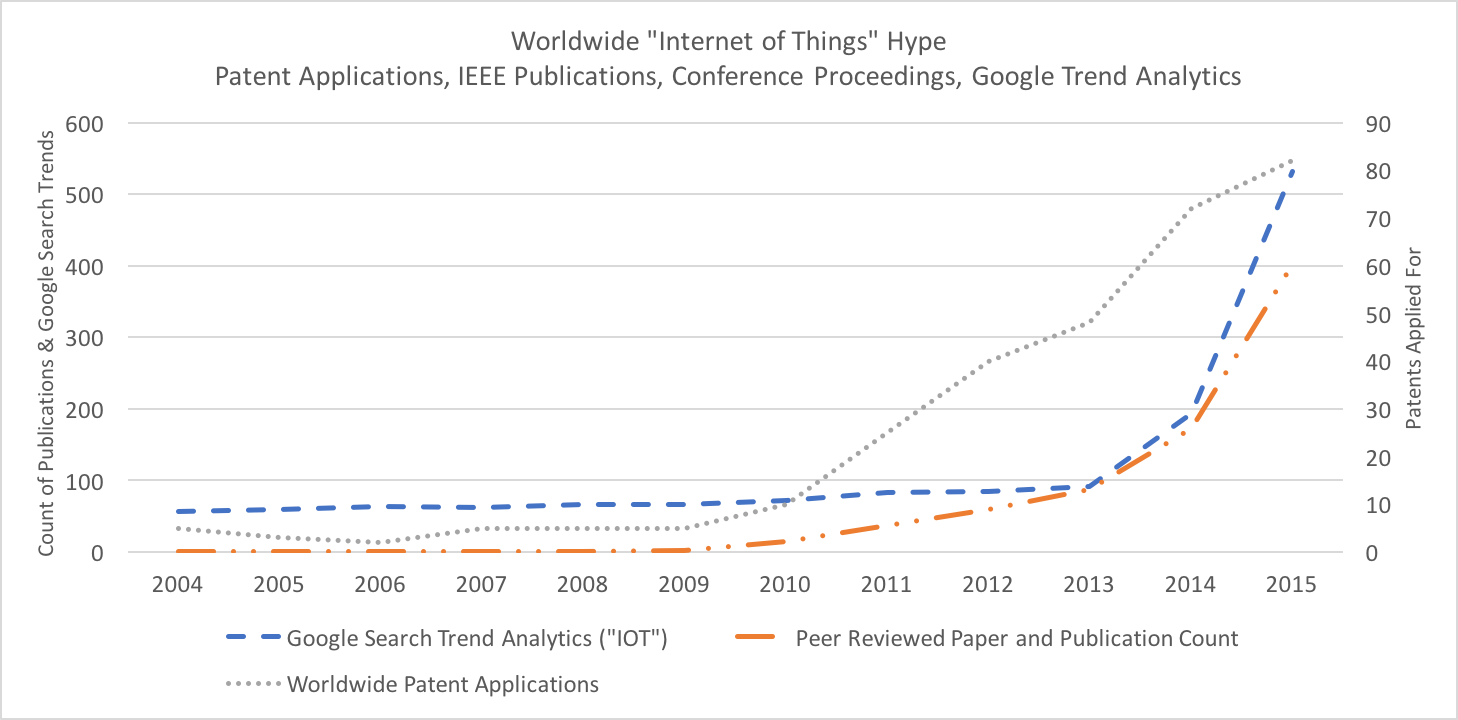
\includegraphics[width=\textwidth]{iot-hype.png}
		\caption{Rosnące zainteresowanie Internetem Rzeczy \cite{iotArchitects}}
		\label{fig:iot-hype}
\end{figure}

Podczas wyboru technologii, na etapie analizy dostępnych rozwiązań okazuje się, że istnieje bardzo wiele podejść do tematu, z których duża część powstała w ciągu kilku ostatnich lat i od momentu publikacji zdobyła natychmiastową popularność. Dodatkowo wszystkie materiały, które pozwoliłyby to wszystko zrozumieć, występują w języku angielskim, najczęściej w kontekście wybranego specjalistycznego zastosowania. 

Powyższy problem przyczynia się do braku zrozumienia technologii chmurowych jako całości. Powoduje to niską świadomość tego, jak w pełni wykorzystać możliwości chmury w kontekście tworzenia typowego projektu informatycznego, jakim jest aplikacja mobilna.





\section*{Cel pracy}
\addcontentsline{toc}{section}{Cel pracy}


Celem pracy było rozstrzygnięcie, jak na obecny stan wiedzy podejść do problemu realizacji typowego projektu aplikacji mobilnej w oparciu o Cloud Computing. W rozumieniu niniejszej pracy, typowa aplikacja pozwala na wprowadzanie i otrzymywanie danych od serwera za pomocą udostępnionego API. W rezultacie miała zostać wybrana konkretna technologia, która pod względem teoretycznym najlepiej odpowiadałaby stawianym wymaganiom.

Wybrana technologia miała zostać użyta w praktyce do stworzenia aplikacji na system Android, komunikującej się z API udostępnianym przez chmurę. Aplikacja miała umożliwiać zapisywanie wydatków w sposób uwzględniający wydatki kilku osób w gospodarstwie domowym. System miał pozwolić założyć konto w serwisie, a następnie połączyć konta w grupy odpowiadające gospodarstwu domowemu. Kategorie wydatków miały pozwolić na uzgodnienie, kto ile płaci w danej kategorii (np. wydatki na higienę po 50\%). Serwer miał być potrzebny do wspomagania rozliczeń pomiędzy poszczególnymi osobami przez dynamiczne naliczanie kto ma ile do oddania. Ponadto miał wspomagać kontrolę własnych wydatków przez uwzględnienie, że koszty życia to nie tylko pieniądze wydawane przez siebie samego, ale również wydatki poniesione przez inne osoby prowadzące to samo gospodarstwo domowe. 

Ponieważ tradycyjne programy do zarządzania wydatkami nie posiadają wyżej wymienionych funkcjonalności, jak również zazwyczaj mogą działać bez serwera, to jest przykład aplikacji, która może nagle stać się popularna i powinna być w stanie wówczas obsłużyć większe obciążenie serwera. 



\section*{Opis rozdziałów}
\addcontentsline{toc}{section}{Opis rozdziałów}
\textit{Rozdział 1. -- Wprowadzenie} zawiera najważniejsze informacje o tym, skąd wziął się Cloud Computing, jaki jest obecny stan wiedzy na jego temat oraz w jakim kierunku zmierza jego rozwój. 

\noindent
\textit{Rozdział 2. -- Porównanie różnych podejść} prezentuje dziewięć różnych podejść do wytwarzania w chmurze serwisów, z którymi może komunikować się aplikacja mobilna. Przy każdym podejściu czytelnik znajdzie listy konkretnych narzędzi oraz usług chmurowych, a także listy zalet i wad danego podejścia.


\clearpage{\pagestyle{empty}\cleardoublepage}
\chapter{Wprowadzenie}

Niniejszy rozdział wyjaśnia, w jaki sposób ewoluowały technologie, by dać się później poznać jako Cloud Computing, a także czego należy oczekiwać od współczesnej chmury. Na końcu rozdziału opisano dokąd zmierza rozwój przedstawionych technologii.



\section{Charakterystyka Cloud Computingu}

Cloud Computing to model, zgodnie z którym wszelkie zasoby informatyczne (oprogramowanie, przestrzeń dyskowa, dostęp do bazy danych itp.) dostarczane są w formie usługi. Istotną cechą jest wysoka \textbf{skalowalność} udostępnianych rozwiązań. Po stronie klienta ma to wyglądać tak, jak gdyby posiadał dostęp do nieskończonej mocy obliczeniowej i niekończącej się przestrzeni dyskowej, natomiast po stronie usługodawcy podłączenie nowych serwerów w celu podtrzymania tej iluzji nie powinno stanowić problemu. \cite{ccBiznes}

\begin{figure}[h]
	\centering
			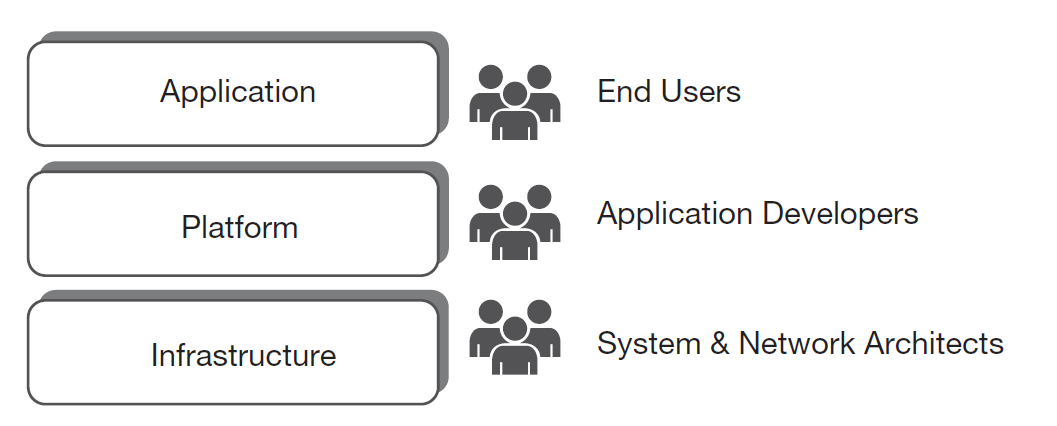
\includegraphics[width=0.7\textwidth]{layers-and-users.png}
		\caption{Różni użytkownicy chmury operujący na jej różnych warstwach \cite{ccCambridge}}
		\label{fig:layers-and-users}
\end{figure}

Aby była możliwa tak wysoka elastyczność, fizyczne serwery są oddzielone warstwą abstrakcji, na której są widoczne jako \textbf{pula zasobów} takich jak przestrzeń dyskowa czy moc procesora (rysunek \ref{fig:pooling}). Każdy program czy serwer wirtualny działający w chmurze osadzany jest na wirtualnych zasobach; nie ma możliwości zdecydowania z którego konkretnego fizycznego zasobu chce się korzystać. Moc chmury obliczeniowej buduje się przez łączenie tanich, łatwo wymienialnych komponentów sprzętowych, w potężne zasoby wirtualne. \cite{ccCambridge}

\begin{figure}[h]
	\centering
			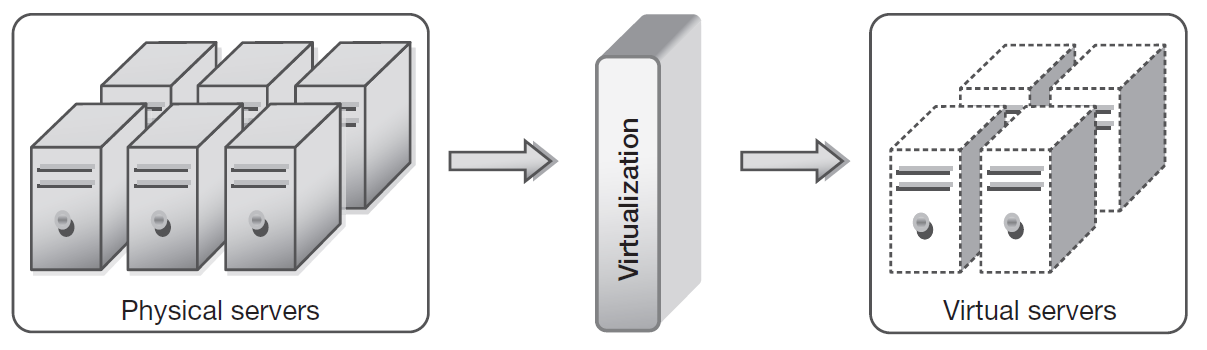
\includegraphics[width=0.7\textwidth]{pooling.png}
		\caption{Serwery wirtualne korzystające z puli zasobów \cite{ccCambridge}}
		\label{fig:pooling}
\end{figure}

Poza rozwiązaniem problemu zarządzania ogromną ilością fizycznych serwerów, wirtualizacja zasobów pozwala na \textbf{lepsze wykorzystanie sprzętu}. W tradycyjnym modelu komputery muszą być przygotowane na wypadek gdyby zainstalowane na nich programy powodowały większe zużycie zasobów. Dzieje się tak nawet w przypadku komputerów PC -- kupuje się specjalnie większe dyski i lepszy procesor, aby przydały się w przyszłości. W ten sposób wykorzystuje się niewielką część możliwości pojedynczego komputera, ponieważ przez większość czasu potrzeba mu znacznie mniej zasobów, niż fizycznie posiada. W przypadku wirtualnych zasobów, do fizycznej jednostki można dynamicznie przypisać zużycie powodowane przez wielu użytkowników, wiele wirtualnych systemów operacyjnych, w zgodzie z ustalonym algorytmem. Algorytm może definiować, że np. wszystkie komputery mają zostać obciążone po równo (round robin), czy że pojedynczy węzeł ma być wykorzystany w 100\% \cite{cloudFoundry}. Technikę tę nazywa się \textbf{równoważeniem obciążenia} (ang. \textit{load balancing}).

Technika zrównoważonego obciążenia przynosi kilka ważnych korzyści, będących istotnymi cechami chmur obliczeniowych. Dzięki niej usługi działające w chmurze mogą być uruchomione na różnych węzłach, w tylu instancjach, ile wymagane jest do prawidłowego obsłużenia ruchu. W przypadku awarii którejś z instancji, użytkownicy usługi niczego nie odczuwają, gdyż zostają przekierowani na instancję co do działania której nie wykazano błędów. Wszystko to ułatwia tworzenie wysoce skalowalnego oprogramowania. Nie bez znaczenia jest także pozytywny wpływ na środowisko naturalne, ponieważ chmury obliczeniowe oznaczają optymalne zużycie istniejącego sprzętu komputerowego, więc nie trzeba produkować go więcej niż potrzeba ani niepotrzebnie zużywać energii elektrycznej.

Najbardziej spektakularne efekty wykorzystywania modelu chmury widać w przypadku dostawców posiadających największe centra danych na świecie, takich jak Amazon, Microsoft, Google czy IBM. Na kilkudziesięciu $m^{2}$ gromadzą zasoby komputerowe, których równocześnie mogą używać miliony osób na całym świecie. Na jednym fizycznym komputerze zasoby mogą być wykorzystywane przez wiele osób niewiedzących o sobie nawzajem (po angielsku tę właściwość określa się jako \textit{multi-tenancy}). Chmury o takiej architekturze mają potencjał ucieleśnić ideę, zgodnie z którą zasoby komputerowe mogą być dostarczane jako usługa użyteczności publicznej.

Wyżej wymieniony sposób myślenia o chmurze jest tym, co wyraźnie odróżnia chmury publiczne od chmur prywatnych. Nic nie stoi na przeszkodzie, aby samemu stworzyć prywatną sieć opartą o model chmury. Wówczas formalnie jest to chmura, lecz nie zapewnia niektórych ważnych korzyści, głównie przez konieczność samodzielnego administrowania serwerami, mniejszą ilość potencjalnych użytkowników oraz mniejszy potencjał puli zasobów. Przykładowo, jeśli firma nadal musi martwić się o zarządzanie fizycznymi jednostkami komputerowymi, to nie będzie miała możliwości wychwalać modelu chmury za brak konieczności zatrudniania specjalistów zajmujących się infrastrukturą komputerową.

\begin{figure}[h]
	\centering
			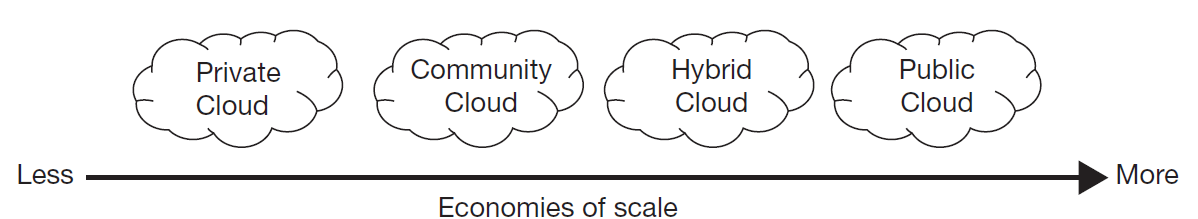
\includegraphics[width=\textwidth]{ekonomia-skali.png}
		\caption{Ekonomia skali rosnąca wraz z ilością użytkowników chmury \cite{ccCambridge}}
		\label{fig:ekonomia-skali}
\end{figure}

\subsection*{Korzyści i wady}

Do głównych korzyści wynikających ze stosowania modelu chmury należą:
\begin{itemize}
\item \textbf{rozwiązanie problemu skalowania aplikacji }\\
Wraz z rozwojem Web 2.0, dostępnością szybkiego łącza internetowego, zwiększaniem ilości urządzeń podłączonych do Internetu oraz ilości transmitowanych danych, istnieje rosnące zapotrzebowanie na aplikacje będące w stanie obsłużyć duży ruch. Dzięki chmurom uruchomienie wielu instancji aplikacji na różnych węzłach, dodatkowo w odmiennych wersjach, sprowadza się do opisu -- ile, w jakiej wersji, w jakich proporcjach.\cite{kubernetesOreily} Podobnie ułatwione jest korzystanie z baz NoSQL.

\item \textbf{rozwój Big Data} \\
Chmury są w stanie zapewnić odpowiednie środowisko do przechowywania oraz przetwarzania dużych zbiorów danych. Udostępnienie tego środowiska jako usługi znacząco redukuje koszt przechowywania i analizy zbiorów danych, dzięki czemu próg wejścia w owo zagadnienie staje się dużo niższy. Za tym idzie wydajniejsze odkrywanie wiedzy z danych, co może mieć wpływ m.in. na rozwój medycyny.

\item \textbf{ochrona środowiska} \\
W modelu chmury sprzęt komputerowy zostaje wydajniej wykorzystany, w związku z tym jest mniejsze zapotrzebowanie na nowy sprzęt. Również dzięki umieszczeniu kosztownych operacji po stronie chmury, urządzenia klienckie łączące się z chmurą nie muszą być regularnie wymieniane na silniejsze.

\item \textbf{lepsza koncentracja na wybranym zadaniu} \\
Model chmury zwalnia użytkowników z dodatkowych czynności przy realizacji danego zadania. Przykładowo, jeśli komuś jest potrzebny serwer, to z chmurą publiczną nie musi martwić się zakupem sprzętu, zapewnieniem odpowiedniego pomieszczenia czy dostępem do Internetu. Może się zamiast tego skupić na właściwym skonfigurowaniu systemu na serwerze wirtualnym. 

\item \textbf{płatność tylko za rzeczywiste zużycie} \\
Chmura umożliwia rozliczanie na podstawie czasu używania procesora, ilości przesłanych megabajtów czy ilości danych przechowywanych w chmurze. W szczególności zmniejsza to początkowy koszt wdrażania czegokolwiek w chmurze.

\item \textbf{gwarancja jakości usługi} \\
Każdy dostawca usług chmurowych udostępnia klientom SLA (ang. \textit{Service-level aggrements}), w którym zobowiązuje się do utrzymania określonego poziomu niezawodności usług (np. dostępność w 99,9\% przypadków) oraz przewidywanego zachowania w przypadku niedotrzymania zapewnień (np. obniżki cen).

\end{itemize}

Ostatnią korzyścią, a jednocześnie kontrowersją, jest bezpieczeństwo danych w chmurach publicznych. Wysyłanie niejednokrotnie wrażliwych danych w nie do końca określone miejsce budzi obawy. Według autorów specjalistycznych wydawnictw\cite{ccCambridge,ccBiznes} obawy te są niesłuszne -- pozostają zgodni co do opinii, że główni dostawcy usług chmurowych są w stanie zapewnić najwyższy poziom bezpieczeństwa, a fizyczne przechowywanie danych na terenie firmy daje tylko ułudę bezpieczeństwa.

Do potencjalnych wad rozwiązań bazujących na chmurach obliczeniowych należą:

\begin{itemize}

\item \textbf{problem z przenoszeniem aplikacji z jednej chmury na drugą}

Znaczna część usług oferowanych przez największych dostawców usług chmurowych jest dedykowana dla tworzonej przez nich chmury. Oznacza to, że jeśli użytkownik chce mieć możliwość zmiany dostawcy, powinien uwzględnić to przy wyborze narzędzi pracy. Więcej na ten temat można przeczytać w rozdziale 2.

\item \textbf{problemy prawne}

Istnieje ryzyko rozbieżności pomiędzy prawem, do którego dostosowywał się dostawca usług chmurowych, a prawem chroniącym dane w kraju, na terenie którego chce się korzystać z tych usług. 

\end{itemize}


\section{Ewolucja Cloud Computingu}

Cloud Computing nie stanowi odrębnej, nowej technologii -- jest to produkt ewolucji technologii rozwijanych od blisko 50 lat. Prześledzenie historii pozwala na zrozumienie, które koncepcje rzeczywiście wprowadzają nową jakość, a nie są jedynie od dawna istniejącą technologią, tyle że  ubraną w ładnie brzmiące słowo.

%\subsection{Historia technologii chmurowych}

Historia ma początek około lat 70., gdy używano wielkich superkomputerów zwanych \textbf{\textit{mainframe}}. Można było z nich korzystać za pomocą terminali, określanych mianem ,,głupich'' (ang. \textit{dumb terminal}), ponieważ nie posiadały procesora i mogły być używane jedynie do operacji I/O. Jako że z serwera mógł korzystać jeden terminal naraz, serwer ustawiał je w kolejkę i musiały długo czekać na obsłużenie.

W latach 70. terminale zaczęły być wyposażone w mikroprocesory i być określane mianem \textbf{,,inteligentnych terminali''} (ang. \textit{intelligent terminal}). Mogły już partycypować przy uruchamianiu programów, co skróciło czas obsługi i dało początek modelowi klient-serwer.

Dalszy rozwój mikroprocesorów dał początek \textbf{komputerom PC}. Komputery te mogły działać samodzielnie i były znacznie tańsze od mainframe'a.

Pojawiły się również LAN (ang. \textit{local area network}) i WAN (ang. \textit{wide area network}), co umożliwiło łączenie komputerów PC w sieci bez konieczności łączenia z mainframe'm. Powstały sieci \textbf{P2P} (ang. \textit{Peer-To-Peer}).

We wczesnych latach 80. wynaleziono \textbf{systemy rozproszone}. Ponieważ były w stanie przetwarzać dane równolegle, zachwiało to poglądem iż większą moc obliczeniową należy uzyskiwać przez wynajdowanie silniejszych procesorów. Systemy rozproszone wymagały wzmożonej ilości operacji komunikacji, lecz występowało to w parze z rozwojem LAN osiągającym przepustowość 100 Mbps oraz WAN osiągającym 64 kbps.

Następnie powstała koncepcja \textbf{klastrów komputerowych}. Klaster polegał na połączeniu komputerów tego samego typu (homogenicznych) w sieć LAN i wyłonieniu wśród nich zarządcy, który będzie zajmował się przydzielaniem zadań pozostałym węzłom. Gdyby któryś z węzłów miał awarię, to inne mogły przejąć jego zadanie. Dało to początek idei \textbf{puli zasobów}. W klastrze niezawodność osiągało się przez nadmiarowość zasobów.

Główną wadą klastrów była konieczność powierzenia zarządzania klastrem jednemu komputerowi. Stanowił on miejsce, od niezawodności którego zależała niezawodność całej sieci (ang. \textit{single point of failure}). Rozwiązaniem okazały się \textbf{gridy}, w których każdy węzeł posiadał równy priorytet. Klient mógł podłączyć się do dowolnego komputera w gridzie, a ponadto komputery te mogły być różnego typu (heterogeniczne). Wkrótce gridy przeniknęły ze świata naukowego do świata biznesu i zaczynały być łączone przez WAN.

Dotychczas gdy uruchamiało się program na wybranym węźle gridu, to znajdował się na tym węźle dopóki proces nie został zakończony. Stanowiło to problem na drodze do skalowania w czasie rzeczywistym, gdzie na skutek zmienionych potrzeb byłoby dobrze mieć możliwość od nowa zaalokować zasoby bez zakłócania działającej usługi. Problem ten rozwiązała \textbf{wirtualizacja sprzętowa}, za pomocą której zadania były alokowane do maszyn wirtualnych. Technika ta umożliwiła \textbf{\textit{utility computing}}, czyli model, w którym zasoby komputerowe mogą być dostarczane jako usługa, co stanowi serce chmur obliczeniowych. Prekursorem została firma Salesforce.com, która udostępnia oprogramowanie w formie usługi internetowej od 1999 r.

\begin{figure}[h!]
	\centering
	\begin{minipage}[t]{0.33\textwidth}
		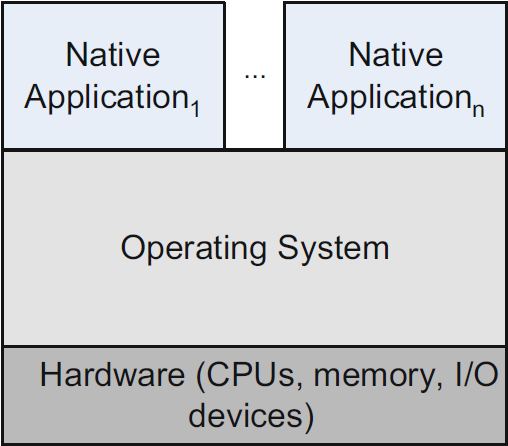
\includegraphics[width=\textwidth]{non-virtualized-system.png}
		\caption{System bez wirtualizacji \cite{ccSpringer}}
		\label{fig:non-virtualized-system}
	\end{minipage}
\hspace*{60px}
	\begin{minipage}[t]{0.33\textwidth}
		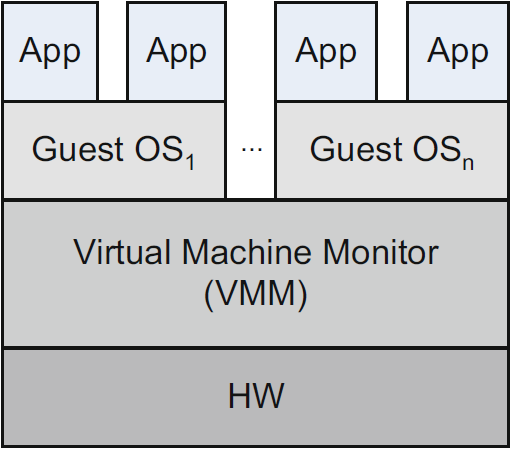
\includegraphics[width=\textwidth]{system-level-vm.png}
		\caption{Wirtualizacja sprzętowa \cite{ccSpringer}}
		\label{fig:system-level-vm}
	\end{minipage}
	\hfill
\end{figure}

W 2001 r. firma IBM zbudowała pierwszy \textbf{autonomiczny system} (ang. \textit{antonomic computing}) -- system, który potrafi sobą zarządzać bez interwencji człowieka. Dzięki wykorzystaniu sztucznej inteligencji do działania, eliminuje się ryzyko związane z błędem ludzkim oraz złożoność związaną z koniecznością doglądania przez człowieka złożonego systemu. IBM wytyczył następujące cechy modelu:
\begin{itemize}
\item automatyczna konfiguracja -- konfiguracja tworzy się automatycznie na podstawie zapotrzebowania,
\item automatyczna naprawa błędów -- system sam wykrywa błędy i reaguje na nie,
\item automatyczna optymalizacja -- system sam dba o optymalne użycie zasobów,
\item automatyczna ochrona -- system wykrywa próby ataków i zapobiega im.
\end{itemize}
Wirtualizacje w tym systemie działają zgodnie z ,,pętlą adaptacyjną'': obserwuj, decyduj, zareaguj.\cite{ccSpringer}


Duże znaczenie miało także wynalezienie metody \textbf{SOA} (ang. service oriented architecture), czyli techniki wytwarzania oprogramowania przez wydzielanie niezależnie działających komponentów, składających się razem na większy system informatyczny. Ważna była również koncepcja \textbf{Web 2.0}, nazwana tak po raz pierwszy w 2002 roku. Model Web 2.0 spowodował zmiany w sposobie myślenia o Internecie, zgodnie z którymi nie powinien jedynie służyć do dostarczania statycznej treści, lecz może być użyteczny również do udostępniania treści tworzonej przez użytkowników Internetu.

Wymienione wyżej technologie zestawione razem dały podwaliny chmurom obliczeniowym.

Przyjmuje się, że termin \textit{,,cloud computing''} po raz pierwszy został użyty przez CEO firmy Google, Erica Schmidta, w trakcie konferencji w 2006 r. Tego samego roku Amazon użył tej nazwy publikując pionierską w swoim gatunku usługę Elastic Compute Cloud (EC2), czyli możliwość wynajmu serwera wirtualnego w ich chmurze.

\section{Historia najnowsza. Współczesne wyzwania}

Odkąd Amazon uruchomił usługę EC2, nastąpił gwałtowny rozwój rozwiązań chmurowych. Praktycznie w tym samym czasie rozwinęły się technologie postrzegane w czasie pisania niniejszej pracy jako rewolucyjne. Na potrzeby opracowania wyróżniono następujące grupy zmian:
\begin{itemize}
\item rozwój chmur publicznych (sekcja \ref{section:chmuryPubliczne}),
\item rozwój rozwiązań opartych o kontenery (sekcja \ref{section:konteneryzacja}),
\item rozwój technik programistycznych wyznaczających najlepsze praktyki tworzenia aplikacji dla chmury (sekcja \ref{section:mikroserwisy}),
\item rozwój technologii bazodanowych dla systemów rozproszonych oraz metod analizy danych (sekcja \ref{section:nosql}),
\item rozwój technologii przyśpieszających dostęp do usług chmurowych (sekcja \ref{section:fog}).
\end{itemize}

\subsection{Rozwój chmur publicznych} \label{section:chmuryPubliczne}

W 2003 roku firma Citrix stworzyła Xen -- system operacyjny przeznaczony tylko do wirtualizacji innych systemów operacyjnych. Niedługo potem Xen został udostępniony jako oprogramowanie otwartoźródłowe. W marcu 2006 r. Amazon na podstawie Xena opracował swój produkt EC2. W ciągu 18 miesięcy zaczęło z niego korzystać ponad pół miliona osób.\cite{ccBiznes}

W kolejnych latach powstały kolejne chmury publiczne oraz nastąpił rozwój rozwiązań typu PaaS (ang. \textit{Platform as a Service}). W czerwcu 2007 r. powstał Heroku, będący pionierem w tej kategorii. Niecały rok później Google udostępnił usługę Google App Engine. W lutym 2010 r. Microsoft udostępnił Windows Azure (w kwietniu 2014 przemianowaną na Microsoft Azure \cite{azurePackt}).

Do tego momentu powstały już 3 największe chmury publiczne: Amazon AWS, Google Cloud Platform, Microsoft Azure. Początkowo miały zróżnicowaną ofertę. W literaturze\cite{ccBiznes} z 2011 r. porównywanie tych platform sprowadzało się do zakresu oferowanych przez nie usług. Z biegiem czasu różnice zatarły się -- obecnie usługa publikowana przez jednego dostawcę po kilku miesiącach jest dostępna także u innych. Tabela \ref{table:historia} prezentuje porównanie tempa rozbudowy zakresu usług.

\noindent
\begin{small}
\begin{table}[t]
\newcolumntype{L}{>{\raggedright\arraybackslash}X}%
\begin{tabularx}{\textwidth}{ |L|L|L|L| }

\hline
\multirow{2}{*}{Typ usługi} & \multicolumn{3}{|c|}{Dostawca} \\

\cline{2-4}
& \multicolumn{1}{|c|}{AWS} & \multicolumn{1}{|c|}{GCP} & \multicolumn{1}{|c|}{Azure} \\

\hline
serwery wirtualne & 2006 -- Amazon EC2 \cite{ccCambridge} & 2013 -- Google Compute Engine \cite{siteGoogleCloudPlatformWiki} & 2010 -- 	Azure Virtual Machines \cite{siteMicrosoftBlogAzure} \\

\hline
platforma aplikacji & 2011 -- AWS Elastic Beanstalk \cite{siteAmazonElasticBeanstalkWiki} &  2008 -- Google App Engine \cite{siteGoogleCloudPlatformWiki} & 2010 -- Azure Cloud Services \cite{siteMicrosoftBlogAzure} \\

\hline
bazy SQL & 2009 -- Amazon Relational Database Service \cite{siteAmazonRdsWiki} & 2011 -- Google Cloud SQL \cite{siteGoogleBlogCloudSql} & 2010 -- Azure SQL Database \cite{siteMicrosoftBlogAzure} \\

\hline
bazy klucz-wartość & 2007 -- Amazon SimpleDb (w 2012 Amazon DynamoDB) \cite{siteAmazonSimpleDbWiki} & 2008 -- Google Bigtable \cite{siteBigTableWikiPl} (jako część App Engine) & 2010 -- Azure Table Storage \cite{siteMicrosoftBlogAzure} (2017 -- Azure Cosmos DB) \\

\hline
serverless & 2014 -- AWS Lambda \cite{serverlessMaddie} & sierpień 2018 -- Google Cloud Functions \cite{siteGoogleServerless} & 2016 -- Azure Functions \cite{serverlessMaddie}\\

\hline
Kubernetes & 2018 -- Amazon Elastic Container Service for Kubernetes \cite{siteAmazonBlogEks} & 2015 -- Google Kubernetes Engine \cite{siteGoogleBlogKubernetes}  & 2017 -- Azure Container Service \cite{siteMicrosoftBlogAks}\\

\hline



\end{tabularx}


\caption{Porównanie dat udostępniania usług chmurowych wśród głównych dostawców}
		\label{table:historia}

\end{table}
\end{small}

\subsection{Konteneryzacja i DevOps} \label{section:konteneryzacja}

W tym samym czasie rozwijały się technologie przeznaczone do wystawiania własnych usług chmurowych. W 2010 r. powstała otwartoźródłowa platforma \textbf{OpenStack} służąca do świadczenia własnych usług typu IaaS. Rok później powstał \textbf{Cloud Foundry} -- również otwartoźródłowy projekt, pozwalający na prowadzenie własnej platformy typu PaaS do tworzenia aplikacji w chmurze. 

Cloud Foundry stanowił odpowiedź na główny problem chmur publicznych -- tworzenie aplikacji na wybraną chmurę wiązało ją z mechanizmami specyficznymi dla tej chmury. Brakowało pomostu, który oddzieliłby warstwę tworzenia aplikacji w chmurze od wybranego usługodawcy, bez konieczności tworzenia serwerów wirtualnych, na których trzeba instalować określone środowisko. \cite{cloudFoundry}

Cloud Foundry jest niezależny od infrastruktury, może działać zarówno na OpenStacku jak i na serwerze wirtualnym w chmurze publicznej. Zapewnia możliwość wyboru dowolnych technologii do wytwarzania oprogramowania. Do działania używa kontenerów zgodnych ze standardem OCI (ang. \textit{Open Container Initiative}). \cite{cloudFoundry} 

\textbf{Konteneryzacja} to metoda wirtualizacji na poziomie systemu operacyjnego, gdzie na działającym systemie operacyjnym można uruchomić wiele odizolowanych od siebie instancji przestrzeni użytkownika. Każda taka instancja to kontener. Kontener zapewnia odpowiednie środowisko do działania dla umieszczonej w nim aplikacji, np. środowisko uruchomieniowe .NET Core w odpowiedniej wersji.  \cite{cloudFoundry,ccSpringer}

\begin{figure}[h]
	\centering
			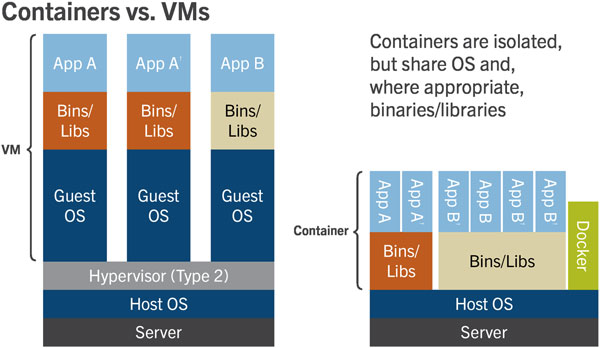
\includegraphics[width=0.7\textwidth]{containers-vs-vms.png}
		\caption{Porównanie serwerów wirtualnych i kontenerów \cite{ccSpringer}}
		\label{fig:containers-vs-vms}
\end{figure}

Cloud Foundry zapewnia orkiestrację kontenerów oraz obsługę procesu CI/CD (ciągłej integracji i ciągłego dostarczania, ang. \textit{continuous integration / continuous delivery}).\cite{cloudFoundry} Stanowi narzędzie pozwalające z powodzeniem wdrażać strategie DevOps. 

\textbf{DevOps} to słowo po raz pierwszy użyte 2009 r. na konferencji w Belgii. Stanowi połączenie ze sobą słów \textit{,,development''} (rozwój) i \textit{,,operations''} (eksploatacja). Wskazuje to na zacieśnianie współpracy pomiędzy zespołami zajmującymi się rozwojem oprogramowania, a zespołami, które je wdrażają. Współpraca ta ma doprowadzać do automatyzacji procesów towarzyszących wytwarzaniu oprogramowania, co w efekcie minimalizuje czas potrzebny od wprowadzenia poprawki do wdrożenia na środowisko produkcyjne, zachowując przy tym niezawodność. Jako strategie DevOps określa się wszelkie technologie i narzędzia inżynierii oprogramowania, które dają taki efekt. \cite{devOpsPackt}

Temat DevOps jest mocno powiązany z chmurami, ponieważ jego koncepcje znacząco redukują złożoność towarzyszącą tworzeniu wysoce skalowalnego oprogramowania. Jednocześnie wychodzą one naprzeciw wymaganiom społeczeństwa coraz bardziej przyzwyczajonego do częstych aktualizacji oprogramowania, szybkiej reakcji na błędy oraz braku przestojów towarzyszących wdrażaniu nowych wersji. W przypadku chmur obliczeniowych, w których jedna usługa internetowa może mieć np. kilkadziesiąt instancji na różnych węzłach, taka automatyzacja ma kluczowe znaczenie. W związku z tym pojęcie DevOps obecnie wchodzi w kanon pojęć związanych z chmurą.

Istotny element DevOps stanowią wcześniej wspomniane kontenery. Idea kontenerów kiełkowała już kilka lat wcześniej, np. Solaris Containers z 2004 r. lub OpenVZ (2005 r.) i LXC (Linux Containers -- 2008 r.), które w istocie do działania wykorzystywały UNIX-owy program chroot z 1982 r.\cite{siteOperatingSystemVirtualizationWiki} Jednak prawdziwe ożywienie spowodowało dopiero pojawienie się Dockera -- sprawił iż tworzenie kontenerów oraz przenoszenie ich pomiędzy systemami stało się łatwe. Na nim bazuje kilka projektów intensywnie rozwijanych w czasie pisania niniejszej pracy.

\textbf{Docker} to system kontenerów, który powstał jako element platformy dotCloud, świadczącej usługi typu PaaS. Spopularyzował się w dość osobliwy sposób. Założyciel myślał, że tylko wygłosi mały referat na PyCon w 2013 r., lecz okazało się, że na konferencji było dużo osób, a jego referat stanowił główny element programu. Do końca roku Docker miał 100 mln pobrań, 3 miesiące później -- 300 mln, a w czerwcu 2017 -- 13 miliardów.\cite{siteDockerHistory} Z kolei platforma dotCloud nie okazała się sukcesem -- w 2014 r. Docker Inc. sprzedał ją niemieckiej firmie cloudControl GmbH, która w grudniu 2015 r. zbankrutowała, a w marcu 2016 r. zamknęła usługę.\cite{siteCloudControlWiki}

Logo Dockera dobrze opisuje jego istotę. Przedstawia wieloryba transportującego kontenery. Miało to nawiązywać do tego, iż załadowanie statku trwa dłużej niż transport statkiem. Ma to swoją alegorię do programowania. W tradycyjnym podejściu, gdyby zechcieć uruchomić np. aplikację napisaną w ASP.NET, najpierw trzeba byłoby poświęcić kilka godzin na pobieranie i instalację narzędzi: Visual Studio z narzędziami sieci Web, serwer IIS oraz SQL Server LocalDB. Natomiast w podejściu Dockera, posiadając zbudowany obraz można by tę aplikację uruchomić od razu. Razem z krokami budowania obrazu byłoby to:
\begin{enumerate}
\item napisanie pliku Dockerfile z definicją zależności: system Windows, MSBuild, .NET Framework, serwer IIS, menadżer pakietów NuGET,
\item użycie CLI Dockera oraz pliku Dockerfile do zbudowania tzw. obrazu Dockera,
\item użycie obrazu Dockera do zbudowania i uruchomienia aplikacji w kontenerze.
\end{enumerate}
Obrazy Dockera działają wszędzie, gdzie jest zainstalowany Docker -- niezależnie od systemu operacyjnego czy środowisk jakie ma zainstalowane. Ponadto zależności takie jak np. system operacyjny Ubuntu występują w wersjach ,,odchudzonych'' - przykładowo obraz Minimal Ubuntu 18.04 zajmuje jedynie 29 MB.\cite{siteUbuntuBlog}. Najlżejszym obrazem Linuxa jest dystrybucja Alpine wielkości niecałych 4 MB, stąd używana jest jako baza dla obrazów zapewnianych przez Docker.\cite{dockerPacktMastering}
Podejście Dockera stwarza następujące możliwości:
\begin{itemize}
\item Na jednej maszynie może jednocześnie działać wiele aplikacji wymagających różnych zależności, lub nawet różniących się jedynie wersjami, w izolacji od siebie oraz maszyny, na której są uruchomione.
\item W procesie wytwarzania oprogramowania gwarantuje użycie identycznych wersji zależności na środowisku deweloperskim, testowym oraz produkcyjnym. Eliminuje to problem, gdy na zgłoszony błąd słyszy się odpowiedź ,,u mnie działa''.
\item Obrazy Dockera są lekkie: współdzielą wiele zasobów systemu operacyjnego, dzielą między sobą inne obrazy Dockera.\cite{siteDockerStackOverflow} Na jednej maszynie może działać wiele kontenerów Dockera, podczas gdy maszyn wirtualnych może być zaledwie kilka.\cite{ccSpringer}
\end{itemize}
Powyższe znacząco ułatwia tworzenie aplikacji ,,dla chmury'', orkiestrację chmury oraz stosowanie strategii DevOps.

W 2014 r. Google udostępnił system \textbf{Kubernetes}, służący do orkiestracji kontenerów w chmurze. Wywodzi się z projektu Borg, będącego wewnętrznym narzędziem Google do obsługi 2 miliardów\cite{kubernetesPacktGettingStarted} kontenerów tygodniowo, dopracowywanym w tej firmie od ponad dekady.\cite{siteKubernetesBlogBorg} Kubernetes jako główny system kontenerów wykorzystuje Dockera.\cite{kubernetesOreily} Kubernetes może zostać skonfigurowany zarówno na fizycznych serwerach, jak i na serwerach wirtualnych (można też je mieszać).\cite{kubernetesPacktMastering}

Na pierwszy rzut oka Kubernetes przypomina Cloud Foundry, jest to jednak zupełnie inne narzędzie. Tabela \ref{table:kubernetes} prezentuje porównanie tych dwóch platform.


\noindent
\begin{small}
\begin{table}[h]
\newcolumntype{L}{>{\raggedright\arraybackslash}X}%
\begin{tabularx}{\textwidth}{ |L|L| }

\hline
Cloud Foundry & Kubernetes \\
\hline
powstał w 2011 r. & powstał w 2014. r. \\
\hline
wysoki poziom automatyzacji -- rozpoznaje zależności aplikacji, sam buduje kontener i konfiguruje skalowanie aplikacji & więcej kontroli nad kontenerami, lecz także więcej pracy dla deweloperów. Dla większej automatyzacji należy sięgnąć po rozwiązania PaaS bazujące na Kubernetes, takie jak RedHat OpenShift \cite{kubernetesPacktGettingStarted} \\
\hline
minimalne wymagania -- 40 GB HDD, 8 GB RAM, 4 rdzenie CPU & 2 GB RAM, 2 rdzenie CPU. Na tyle lekki, że można go używać na Raspberry PI \cite{siteKubernetesOnRaspberry} \\
\hline
domyślnie używa własnego systemu kontenerów, ale pozwala na korzystanie z obrazów Dockera & stosuje obrazy Dockera jako główny system kontenerów, ale pozwala zastąpić go innym \\
\hline


\end{tabularx}


\caption{Główne różnice pomiędzy Cloud Foundry i Kubernetes}
		\label{table:kubernetes}

\end{table}
\end{small}

Do tego momentu kontenery jawią się jako antidotum na przywiązanie do wybranego dostawcy usług chmurowych. Aplikacje w kontenerze Dockera mogą używać szerokiego wachlarza technologii, nie tylko otwartoźródłowych jak np. MongoDB, Node.js, .NET Core. Jako zależność można podać np. OpenJDK czy obraz systemu Windows Server udostępniany przez Microsoft, następnie można do niego doinstalować inne zależności komendą \texttt{RUN} w Dockerfile. \cite{dockerPacktMastering} Dostępność platformy Kubernetes wyznaczyła standard w zarządzaniu kontenerami na szeroką skalę.

Problemem, który w wielu przypadkach mógł podnosić barierę wejścia do stosowania takich rozwiązań, była konieczność samodzielnej instalacji Kubernetes lub podobnego narzędzia na serwerze wirtualnym w chmurze. Chmury publiczne wyszły naprzeciw tym oczekiwaniom i zaczęły udostępniać usługi typu \textbf{CaaS} (ang. \textit{Containers as a Service}), nazywane też KaaS (ang. \textit{Kubernetes as a Service}). Jako przykłady można wymienić:
\begin{itemize}
\item \textbf{Google Kubernetes Engine} (wcześniej: Google Container Engine) -- usługa udostępniona w sierpniu 2015 r. \cite{siteGoogleBlogKubernetes} z gotowym do użycia Kubernetes. Można ją przetestować za darmo w ramach kredytu 300 USD do testowania Cloud Platform.\cite{siteGoogleTry}
\item \textbf{AKS -- Azure Kubernetes Service} (wcześniej: Azure Container Service) -- początkowo od 2015 r. wspierała orkiestratory Mesosphere DC/OS oraz Docker Swarm, jednak na fali popularności Kubernetes firma Microsoft uznała go za standard i w 2017 r. opracowała wsparcie dla Kubernetes. W związku z tym nastąpiła także zmiana nazwy usługi. \cite{siteMicrosoftBlogAks} Usługa jest darmowa\cite{siteAksPricing}, opłaty są naliczane za użyte maszyny wirtualne, które przez rok również w ograniczonym zakresie są bezpłatne.\cite{siteAzureTry}
\item \textbf{Amazon ECS -- Amazon Elastic Container Service} -- usługa dostępna od kwietnia 2015 r., jest to własna implementacja orkiestracji kontenerów Dockera stworzona przez Amazona. Pozwala na 2 typy rozliczeń: płatność za zużycie zasobów przez kontener lub płatność za przechowanie i uruchamianie aplikacji na EC2.\cite{siteAmazonEcsPricing} Nie występuje na liście usług dostępnych do wypróbowania za darmo.\cite{siteAmazonTry}
\item \textbf{Amazon EKS -- Amazon Elastic Container Service for Kubernetes} -- usługa została uruchomiona w czerwcu 2018 roku. Publikując usługę Amazon chwalił się, że na podstawie danych Cloud Native Computing Foundation (założonej wraz z powstaniem Kubernetes), 57\% firm korzystających z Kubernetes robiło to na serwerach wirtualnych AWS. Płatność wynosi 0.20 USD za godzinę dla każdego klastra w usłudze, a dodatkowo za zużycie zasobów AWS.\cite{siteAmazonEksPricing} Nie występuje na liście usług dostępnych do wypróbowania za darmo.\cite{siteAmazonTry}
\end{itemize}

Dostępność tych usług ucieleśnia wizję tworzenia aplikacji dla chmury tak,	 że:
\begin{itemize}
\item Do tworzenia aplikacji można wybrać dowolną technologię i wciąż koncentrować się na tworzeniu tej aplikacji, a nie zapewnianiu jej odpowiedniego środowiska na serwerze wirtualnym.
\item Istnieje standardowy sposób tworzenia obrazu kontenera (Docker).
\item Istnieje standardowy sposób orkiestracji kontenerów (Kubernetes). Wiedzę na temat korzystania z niego można zastosować do projektów działających na chmurach publicznych, prywatnych i hybrydowych.
\end{itemize}

\subsection{Mikrousługi i serverless} \label{section:mikroserwisy}

Gwałtowny rozwój chmur obliczeniowych poskutkował również wytworzeniem nowych wzorców projektowych, wzorców architektonicznych oraz dobrych praktyk używanych podczas tworzenia aplikacji przeznaczonej dla chmury. W chmurze może działać praktycznie każdy program, wszakże odpowiednio przygotowana maszyna wirtualna wszystko przyjmie. Chcąc jednak maksymalnie wykorzystać atuty chmury, a jednocześnie zapewnić niezawodność i jak najniższy koszt eksploatacji, należy zapoznać się ze specyficznym sposobem tworzenia aplikacji dla chmury. Aplikację zgodną z tymi wytycznymi określa się jako \textbf{\textit{cloud native}}.

Jak zostało wspomniane wcześniej, platforma Heroku była pionierem jeśli chodzi o udostępnianie programistom platformy do tworzenia aplikacji w chmurze (2007 r.). Współzałożyciel Heroku, Adam Wiggins wraz z zespołem, w 2012 r. na podstawie doświadczeń zebranych w Heroku stworzyli metodykę \textit{,,twelve-factor''} (ang. \textbf{\textit{The Twelve-Factor App}}). Jest to zbiór podstawowych 12. reguł dotyczących programowania oraz pracy z aplikacjami przeznaczonymi dla chmury. Reguły te są często przywoływane w literaturze zajmującej się tym tematem.\cite{cloudFoundry, microservicesPacktNetCore} Można się z nimi zapoznać odwiedzając stronę \texttt{https://12factor.net} (w czasie pisania pracy strona była dostępna w 13 językach, w tym w języku polskim).

Osobne ,,dobre praktyki'' powstały dla systemów rozproszonych używających kontenerów (w tym Kubernetes). Dzielą się na:
\begin{itemize}
\item Wzorce dla kontenerów występujących na jednym węźle (ang. \textit{Single-node patterns}). Należą do nich wzorce: \textit{Sidecar, Ambassador, Adapter}.
\item Wzorce dla kontenerów występujących na różnych węzłach (ang. \textit{Multi-node patterns}). Koncentrują się na właściwych metodach koordynacji działań pomiędzy różnymi maszynami. Są to wzorce np. komunikacji z użyciem zdarzeń czy kolejek.  \cite{kubernetesPacktMastering, distributedSystems}
\end{itemize}

Praktyki wyznaczone przez powyższe wzorce w dużej mierze opierają się na \textbf{mikrousługach}. Mikrousługi wywodzą się z \textbf{SOA}. Termin SOA (ang. \textit{Service oriented architecture}) został pierwszy raz użyty przez analityka firmy Gartner podczas wykładu. Utworzył on ten termin, ponieważ zwrot ,,klient/serwer'' tracił na swoim pierwotnym znaczeniu, gdyż zamiast nazywać tak aplikację dla serwera lub klienta, ludzie zaczęli tak nazywać fizyczne maszyny. Następnie inni analitycy w 1996 r. publikowali na ten temat raporty. Bardziej znaczące użycie terminu SOA należało do Microsoftu. W 2000 r. opisywał zbiór standardów do komunikacji komputerów przez Internet, gdzie przedstawił architekturę SOA jako ważną, choć nie niezbędną, dla Web Services. Wkrótce termin podchwyciły inne firmy, w tym  takie jak IBM, Oracle, HP, publikując nowe koncepcje czy narzędzia powiązane z SOA. \cite{soaOreily}

SOA to po polsku architektura zorientowana na usługi. Polega na podzieleniu systemu informatycznego na odrębne części, które mogą znajdować się na różnych maszynach i komunikować się ze sobą przez sieć. Główne koncepcje SOA to: 
\begin{itemize}
\item usługi -- rozumiane jako samodzielne komponenty realizujące daną funkcjonalność biznesową,
\item wysoka interoperacyjność -- łatwe łączenie ze sobą systemów różnych typów,
\item luźne wiązania -- jak najmniejsza liczba zależności. \cite{soaOreily}
\end{itemize}

SOA to bardzo ogólne pojęcie, nie definiuje jakiej wielkości powinny być poszczególne usługi. Wraz z rozwojem technologii chmurowych, nastała potrzeba dostosowania paradygmatu SOA do wyzwań związanych ze skalowalnością, szybkością wytwarzania oprogramowania oraz potrzebą adaptacji nowych technologii dla istniejących rozbudowanych systemów. Odpowiedzią na ten problem okazały się mikrousługi.

\textbf{Mikrousługi} (ang. \textit{microservices}) stanowią szczególny przypadek SOA. Ich główna cecha: mają być małe. Zamiast tworzyć jedną aplikację, która robi wszystko, system ma składać się z wielu małych, niezależnych od siebie komponentów, odpowiedzialnych za tylko jedną rzecz. \cite{microservicesPacktNetCore}

Z jednej strony powinny grupować powiązane ze sobą funkcjonalności, z drugiej strony nie wolno doprowadzać do sytuacji, gdy serwis może stać się zbyt duży i trudny w utrzymaniu. Pomocne w wyobrażeniu jakiej wielkości powinna być przeciętna mikrousługa są następujące wskazówki:
\begin{itemize}
\item Zasada pojedynczej odpowiedzialności, wywodząca się z zasad SOLID, a zaadoptowana do usług. Polega na umieszczaniu razem elementów, które będą zmieniać się z tego samego powodu. \cite{microservicesWmii}
\item Kod mikrousługi powinien być na tyle mały, żeby dało się go przepisać w dwa tygodnie. \cite{microservicesWmii}
\item Mikrousługa powinna być na tyle mała, żeby do pracy z nią wystarczył jeden zespół programistów. \cite{microservicesSusan}
\item W przypadku gdy mikrousługa jest często używana i potrzebuje do działania wielu instancji, nie powinna jednocześnie powielać funkcjonalności rzadziej używanych i tym sposobem marnować zasobów. \cite{microservicesSusan}
\end{itemize}

W odniesieniu do chmur, mikrousługi wprowadzają następujące udogodnienia: \cite{microservicesPacktNetCore, microservicesSusan, microservicesWmii}
\begin{itemize}
\item \textbf{Efektywne skalowanie.} Gdy określona funkcjonalność systemu jest często używana, uruchamia się więcej instancji mikrousługi odpowiedzialnej za tę funkcjonalność. Nie trzeba zużywać więcej zasobów niż jest to potrzebne.
\item \textbf{Lepsze zapanowanie nad kodem.} Do mniejszego programu łatwiej wprowadzać poprawki, w razie potrzeby przepisanie go do nowszych technologii nie powinno stanowić problemu. Każda mikrousługa może być napisana przy użyciu innych technologii. Większe zmiany w kodzie oddziałują tylko na daną mikrousługę, nie na cały system.
\item \textbf{Szybsze wdrażanie.} Procesy ciągłej integracji i ciągłego dostarczania (CI/CD) szybciej działają, gdy mają do kopiowania, budowania i testowania mniejszą ilość kodu. 
\end{itemize}

Popularność kontenerów, mikrousług oraz modelu \textit{utility computing} (rozliczanie za rzeczywiste użycie zasobów komputerowych) doprowadziła do wytworzenia nowego paradygmatu tworzenia aplikacji w chmurze, znanego jako \textbf{\textit{serverless}} (z ang. ,,bez serwera''). Serverless jest obecnie obiecującą nowością jeśli chodzi o przetwarzanie w chmurze. Nazwa ta zaczęła zdobywać popularność na początku 2016 r. \cite{ccResearchSpringer}  

Aplikacje tego typu zamiast być przez cały czas uruchomione na serwerze w oczekiwaniu na zapytania, mają być uruchamiane dopiero gdy przyjdzie określone zdarzenie (ang. \textit{event-driven computation}). Zdarzeniem może być np. nowe zapytanie HTTP, nowy wpis w kolejce, wywołanie po upłynięciu interwału czasowego. Wówczas zostaje powołana do życia aplikacja przeznaczona tylko do obsługi danego zdarzenia i działa tylko na krótki czas obsługi zdarzenia (jest to maksymalnie około kilka minut). Aplikacje te to w istocie mikrousługi, tyle że posiadające tylko jedną funkcję -- stąd nazywa się je po prostu funkcjami. Dla lepszego odróżnienia od mikrousług określa się je jako ,,nanousługi'' (ang. \textit{nanoservices}). \cite{serverlessMaddie, ccResearchSpringer, distributedSystems}

Platforma w chmurze stosująca model serverless określana jest jako \textbf{FaaS} (ang. \textit{Function as a Service}). Pierwszym znaczącym dostarczycielem tej usługi był Amazon -- już w 2014 r. uruchomił usługę AWS Lambda typu FaaS. W 2016 r. Microsoft udostępnił usługę Azure Functions. W Google Cloud Platform tego typu usługa została oficjalnie udostępniona w sierpniu 2018 (miesiąc przed wydaniem niniejszej pracy), choć wersja poglądowa była dostępna wcześniej. 

Posługując się modelem serverless, usługodawca może stosować rozliczenie według ilości wywołań poszczególnych funkcji. Dzięki temu nie trzeba płacić za programy bezczynnie czekające na przychodzące zapytania.

Dla programisty użycie nanoserwisów oznacza mniej projektowania, jeśli chodzi o optymalną architekturę mikrousług. Mikrousługi grupowały ze sobą niektóre elementy, natomiast w nanousługach każda funkcja stanowi osobny byt. Według Maddie Stigler, autorki książki \textit{,,Beginning Serverless Computing''}, użycie architektury serverless oszczędza połowę czasu potrzebnego na stworzenie skalowalnych aplikacji od podstaw.\cite{serverlessMaddie}

Rozwijane są także inicjatywy niezwiązane z usługami FaaS konkretnych dostawców. W 2015 r. powstał projekt Serverless Framework,\cite{siteServerlessFramework} służący do odseparowania logiki konkretnej usługi FaaS od logiki biznesowej funkcji. Ponadto zapewnia narzędzia wspierające proces tworzenia funkcji. 

W 2017 r. powstał projekt Kubeless.\cite{siteKubelessReleases} Jest to otwartoźródłowy framework dla Kubernetes, który ma działać w sposób podobny do sposobu wyznaczonego przez AWS Lambda, Azure Functions oraz Google Cloud Functions.\cite{distributedSystems} 

Serverless Framework obsługuje wszystkie wyżej wymienione platformy, z Kubeless włącznie.\cite{siteServerlessFramework}


\subsection{Bazy NoSQL, NewSQL i rozwiązania dla Big Data} \label{section:nosql}

W literaturze rozróżnia się trzy rewolucje w rozwoju technologii bazodanowych.  \cite{noSqlHistory} W niniejszej sekcji zostaną przytoczone wszystkie trzy, ponieważ pokazuje to, jak kiedyś wyglądały bazy nierelacyjne (teraz postrzegane jako nowość), jak bardzo długo nie było potrzeby rezygnowania z relacyjnych baz danych, oraz jak na tym tle prezentuje się tempo rozwoju współczesnych baz danych.

Za pierwsze ,,bazy danych'' uznaje się wszelkie techniki zapisu i odczytu danych z nośników, na które pozwalała technika -- kart perforowanych, taśm magnetycznych, magnetycznych dysków twardych. Przed pierwszą rewolucją, każda aplikacja posiadała swoją własną implementację dostępu do danych. Nie istniały żadne mechanizmy chroniące przed uszkodzeniem danych, przed równoczesnym dostępem wielu użytkowników, nie wspominając o optymalizacjach. 

Pierwszą rewolucją było stworzenie \textbf{systemu bazodanowego} (\textbf{DBMS} -- ang. \textit{Database Management System}). Wczesne systemy nie opierały się na żadnych podstawach matematycznych. Były to tzw. bazy nawigacyjne, gdzie relacje uzyskiwało się definiując połączenia pomiędzy obiektami. Struktura projektu definiowała jakie będzie można tworzyć rodzaje zapytań do bazy. Przykłady tych wczesnych baz stanowią: IMS od firmy IBM (typ hierarchiczny) oraz IDMS będący implementacją standardu CODASTYL (typ sieciowy). 

Drugą rewolucję zaczął Edgar Codd, będący matematykiem-programistą oraz wieloletnim pracownikiem firmy IBM. Był on pierwszą osobą, która zwróciła uwagę na wady istniejących rozwiązań wynikające z braku podstaw matematycznych, i w 1970 r. opublikował artykuł opisujący relacyjne bazy danych. Początkowo pozostał on bez odzewu. Dopiero w 1974 r. IBM zaczął prace nad prototypem zwanym Systemem R. Prototyp był gotowy w 1976 r. Poza modelem opracowanym przez Codd'a, na potrzeby systemu stworzono język SQL do tworzenia zapytań do bazy danych oraz opracowano zasady obsługi równoległych zapytań. Jim Gray zdefiniował transakcje ACID.

Pierwszą komercyjną \textbf{relacyjną bazą danych} (\textbf{RDBMS} - \textit{Relational Database Management System}) była Oracle Database. Założyciel Oracle, Larry Ellison, był zaznajomiony zarówno z pracą Codd'a, jak i Systemem R. Wierząc w relacyjne bazy danych, w 1979 r. wydał pierwszą na świecie komercyjną relacyjną bazę danych obsługującą język SQL. \cite{relationalDbs}

W tym samym czasie (od roku 1977) pionierski stał się również projekt Ingres, stworzony przez Michaela Stonebraker'a. Początkowo jako język zapytań stosował QUEL, popularność bazy Oracle wymusiła jednak konieczność obsługi SQL. W połowie lat 80. na bazie Ingres powstał projekt Postgres (post-ingres), znany dzisiaj jako PostgreSQL. 

Po sukcesie Oracle IBM opublikował komercyjną bazę SQL/DS w 1981 r. W późniejszych latach powstawały inne relacyjne bazy chętnie stosowane do dziś: Microsoft SQL Server, PostgreSQL, MySQL. Wszystkie te bazy co do zasady są do siebie podobne -- opierają się o model Codd'a, transakcje ACID oraz język SQL. \cite{relationalDbs}

Potencjalna rewolucja miała szanse dokonać się po latach 80., gdy zaczął popularyzować się paradygmat programowania obiektowego. Istniejące języki zaczęły występować w wersji obiektowej, np. Object Pascal, powstały języki od początku obiektowe, np. Java. Niektórym programistom nie podobała się rozbieżność pomiędzy reprezentacją danych w obiekcie, a w relacyjnej bazie danych. W grudniu 1989 r. powstał manifest obiektowych baz danych (OODBMS, ang. \textit{Object Oriented Database Management System}), w którym bazy relacyjne jawiły się jako relikt przeszłości, a obiektowe jako ich następcy.\cite{oodbmsManifesto} Jednak na przestrzeni lat 90. okazało się, że bazy obiektowe nie zdobyły rynku, nawet pod postacią nowych opcji w popularnych bazach jak np. Oracle. Według Guy'a Harrison'a, autora książki \textit{,,Next Generation Databases: NoSQL, NewSQL, and Big Data''}, założenia baz obiektowych koncentrowały się wokół korzyści dla programisty, ignorując korzyści dla biznesu (np. brak wsparcia dla języka SQL będącego powszechnie w użyciu). Dodatkowo dostępność narzędzi ORM (ang. \textit{Object-relational mapping}) znacząco ułatwiła korzystanie z RDBMS w językach obiektowych, więc bazy relacyjne przestały irytować.

\subsubsection{Trzecia rewolucja}

Trzecia rewolucja rozpoczęła się za sprawą coraz większego znaczenia systemów rozproszonych oraz konieczności analizy dużej ilości danych. Zaczęło się od Google. W 1996 r. powstała wyszukiwarka Google, korzystająca z algorytmu PageRank. W 2005 r. Google był największą stroną internetową na świecie, stroną zbierającą i przetwarzającą dane o wszystkich innych stronach. Potrzebowano nowych narzędzi do rozwiązania problemu, z którym jako pierwsi mieli styczność. W kolejnych latach Google publikował szczegóły swoich rozwiązań, co miało duży wpływ na rozwój dalszych technologii:
\begin{itemize}
\item w 2003 r. -- system plików \textbf{GFS} (Google File System) dla systemów rozproszonych, gdzie pula zasobów dyskowych jest widoczna jako jedno,
\item w 2004 r. -- model \textbf{MapReduce} pozwalający na przetwarzanie danych w systemach rozproszonych,
\item w 2006 r. -- baza danych \textbf{BigTable}.
\end{itemize}
Ponadto w 2005 r. Google opatentował Modular Data Center, czyli sposób na szybką rozbudowę centrum danych. Zamiast z osobna dodawać serwery, mogli dodawać od razu po tysiąc naraz.

Rozwiązania Google zainspirowały inne projekty. W 2004 r. powstał projekt Apache Nutch, który miał być otwartoźródłową wyszukiwarką internetową. Gdy Google opublikował GFS i MapReduce, dla Nutch to był sygnał jak rozwiązywać problemy skalowalności. W 2006 r. Yahoo! zainwestował w projekt, pomimo że był otwartoźródłowy, ponieważ chciał użyć go w swoim produkcie. Adaptację rozwiązań Google wyodrębniono jako osobny projekt. Tak w 2007 r. powstał \textbf{Apache Hadoop}. \cite{hadoop}

Hadoop to nie tylko projekt, ale podejście do skalowalnego przetwarzania danych. \cite{hadoop} Obecnie Hadoop to praktycznie synonim Big Data. \cite{bigData} Termin \textbf{Big Data} (z ang. ,,duże dane'') po raz pierwszy został użyty w 1999 r., jednak zaczął być powszechnie używany odkąd Google użył tego terminu w dokumencie opisującym MapReduce w 2004 roku. Początkowo (w 2001 r.) opisywano Big Data za pomocą ,,trzech \textit{V}'': \textit{volume, variety, velocity} (ilość, różnorodność, szybkość). W 2014 r. rozszerzono to do ,,pięciu \textit{V}'' o: \textit{veracity, value} (wiarygodność, wartość).\cite{realTimeProcessing} Właściwości te wyznaczają obszar zainteresowań, gdzie zastosowanie mają takie narzędzia jak Hadoop:
\begin{itemize}
\item \textit{volume} -- ilość danych,
\item \textit{variety} -- stopień różnorodności źródeł danych,
\item \textit{velocity} -- szybkość z jaką są tworzone nowe dane oraz jak szybko należy je przetworzyć,
\item \textit{veracity} -- na ile można ufać tym danym, czy źródło danych jest zanieczyszczone,
\item \textit{value} -- czy dane mają jakiekolwiek znaczenie, czy analiza tych danych tylko tworzy koszty czy daje wartość.
\end{itemize}
Powyższe oznacza, że wcale nie trzeba mieć bardzo dużego zbioru danych, aby potrzebować Big Data. \cite{hadoop}

Wracając do Hadoopa, rok po jego wdrożeniu Yahoo! ogłosił, że ich klaster Hadoopa ma 5 petabajtów dysku i ponad 10 000 rdzeni CPU, co generowało im cały indeks wyszukiwarki. Podobnie Facebook skorzystał z Hadoopa w 2007 r. i już w 2008 r. mieli 2500 rdzeni CPU, a w 2012 r. 100 petabajtów dysku, co wyparło użycie rozwiązań Oracle w tej firmie.

Do głównych zalet Hadoopa zalicza się:
\begin{itemize}
\item tanie przechowywanie danych -- jest to możliwe na zwykłych dyskach,
\item skalowanie operacji I/O -- ponieważ zamiast dodawać tylko dyski, dodaje się nowe komputery,
\item niezadowność -- jeśli zepsuje się jeden komputer, to jego rolę przejmie inny,
\item \textit{,,schema on read''} -- struktura danych tworzy się podczas czytania źródła danych, w przeciwieństwie do tradycyjnego modelu relacyjnego, gdzie przy zapisie danych należy się zastosować do istniejącego schematu (ang. \textit{schema on write}).
\end{itemize}

Klasyczny Hadoop posiadał ograniczenia jeśli chodzi o użycie innego modelu przetwarzania zadań niż MapReduce. W 2012 r. powstała wersja 2.0, w której dołączono platformę YARN (ang. \textit{Yet Another Resource Negotiator} lub rekursywnie \textit{YARN Application Resource Negotiator}). YARN pozwala na użycie MapReduce jako jednego z możliwych frameworków do zastosowania. Zamiast niego można użyć np. Sparka, pozbawionego niektórych niedogodności MapReduce (krótkotrwałość zadań, brak możliwości trzymania roboczego zbioru danych w pamięci). \cite{hadoop, bigData}

Stworzenie BigTable oraz Hadoopa spowodowało powstanie wielu nowych systemów bazodanowych, które miały lepiej działać na systemach rozproszonych. Dzielą się na:
\begin{itemize}
\item \textbf{Bazy NoSQL} -- bazy nierelacyjne. Zalicza się do nich wszelkie rozwiązania, które dzięki niespełnieniu niektórych reguł ACID mogą pozwolić na lepszą skalowalność i/lub szybkość przetwarzania.
\item \textbf{Bazy NewSQL} -- bazy posiadające możliwość skalowania, zachowujące właściwości ACID baz relacyjnych.
\end{itemize}

W 2005 r. Michael Stonebraker (założyciel Ingres i PostgreSQL) opracował bazę C-Store, postulującą \textbf{model kolumnowy}. Pomysł opiera się o tradycyjną relacyjną bazę danych, gdzie w tabeli zostają zamienione miejscami wiersze z kolumnami. Taka zamiana powoduje szybsze działanie zapytań agregujących, gdyż wszystkie potrzebne dane znajdują się obok siebie. Poza tym, ponieważ obok siebie znajdują się dane bardzo podobnej postaci, można zastosować lepszą kompresję, nawet przez traktowanie każdej kolejnej danej jako zmianę względem poprzedniej.

W 2007 r. Amazon opracował bazę Dynamo, która stała się wzorcem dla baz w modelu \textbf{klucz-wartość}. Jedną z nich jest Apache Cassandra (2008 r.), baza typu \textit{\textbf{wide-column}}. W bazach tego typu w miejscu wartości jest dynamiczna liczba kolumn, co pozwala np. na przeszukiwanie po danej kolumnie lub aktualizację tylko danej kolumny, zamiast całego obiektu. Podobnym projektem jest Apache HBase (2008 r.).

Również w 2007 r. powstała pierwsza \textbf{baza dokumentowa}, która mogła być postrzegana jako alternatywa dla RDBMS. Od 2000 r. powstawały bazy XML, ale raczej mające na celu zarządzanie już istniejącymi dokumentami w tym formacie. XML rozpowszechniał się za sprawą popularności AJAX, później w tej technice zaczął być zastępowany formatem JSON. Takie dane były już formą dokumentu, a stworzenie systemu do przechowywania ich było kwestią czasu. W 2005 r. powstała baza dokumentowa Apache CouchDB, na razie obsługująca XML, a w 2007 r. była to pierwsza znacząca baza dokumentów JSON. W 2009 r. powstała baza MongoDB, przechowująca dokumenty JSON (wewnętrznie zapisywane jako BSON -- \textit{Binary JSON}). Stanowi dziś najpopularniejszą bazę tego typu.

Kolejnym osiągnięciem z 2007 r. był artykuł Michaela Stonebrakera pt. ,,The end of an architectural era: (it's time for a complete rewrite)'' (,,Koniec współczesnych architektur, czas przepisać je na nowo'' -- tłumaczenie własne). Opisał tam koncepcję bazy H-store typu \textit{\textbf{in-memory}}, która do transakcji nie potrzebuje wykonywać operacji I/O na dysku. Pomysł opiera się na lepszym wykorzystaniu pamięci RAM i dysków SSD. Komercyjną implementacją tego pomysłu była baza VoltDB, utworzona w 2008 roku. Jest to baza typu NewSQL.

Rok 2007 był przełomowy także dla modelu \textbf{baz grafowych} -- powstała wtedy baza Neo4J. Bazy grafowe przypominają wczesne, nawigacyjne bazy danych, lecz operują na wyższym poziomie abstrakcji oraz pozwalają na przeszukiwanie grafu do zadanego poziomu. Są stworzone dla danych, gdzie najważniejszą właściwością są relacje z innymi danymi, np. relacje w social media. Do odpytywania bazy grafowej używa się języków Cypher oraz Gremlin. Neo4J stanowi bazę czysto grafową, jednak nie obsługuje systemów rozproszonych, gdyż łączenie wierzchołków grafu z różnych serwerów znacząco obniżyłoby jego wydajność. Do projektów przetwarzania grafów na systemach rozproszonych należą: Apache Giraph (2016 r.), GraphX (część Apache Spark, 2014 r.), Titan (2015 r.) -- działający jako nakładka na HBase czy Cassandrę.


\subsection{CDN i Fog Computing} \label{section:fog}

Jak było wspomniane wcześniej, chmury obliczeniowe gromadzą się co do zasady w gigantycznych centrach danych. Scentralizowany charakter chmur powoduje opóźnienia względem dostępności usług znajdujących się bliżej użytkownika. W celu zapewnienia wysokiej jakości usług (ang. QoS, \textit{Quality of Service}) stosuje się sieci \textbf{CDN} (ang. \textit{Content Delivery Network}). Węzły sieci CDN są szeroko rozpostarte po całym świecie, na krawędzi (ang. \textit{edge}) dostawców usług internetowych (ang. ISP, \textit{Internet service provider}), znacznie bliżej użytkowników końcowych niż odległość od centrów danych (rysunek \ref{fig:cdn-schemat}). \cite{cdn}

\begin{figure}[h]
	\centering
			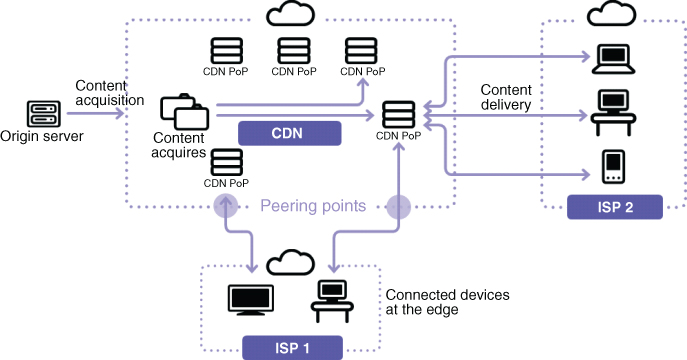
\includegraphics[width=0.7\textwidth]{cdn-schemat.jpg}
		\caption{Schemat sieci CDN. \cite{cdn}}
		\label{fig:cdn-schemat}
\end{figure}

Początkowo większość treści znajdujących się w Internecie była statyczna, więc zadanie sieci CDN koncentrowało się na tworzeniu cache często pobieranej treści. Z czasem treść zaczęła się robić coraz bardziej dynamiczna, zaczęło się upowszechniać strumieniowanie wideo (rysunek \ref{fig:cdn-streaming}). Spowodowało to powstanie drugiej generacji sieci CDN będącej w stanie obsłużyć te przypadki. W technologiach CDN od lat przewodzi założona w 1998 r. firma Akamai. Obecnie posiada ponad 240 000 serwerów CDN w ponad 130 krajach na całym świecie.\cite{siteAkamaiFacts} Do innych znaczących dostarczycieli usług tego typu należą: Limelight, CloudFront (część Amazon AWS), Azure CDN. \cite{ccCambridge, cdn}

\begin{figure}[h]
	\centering
			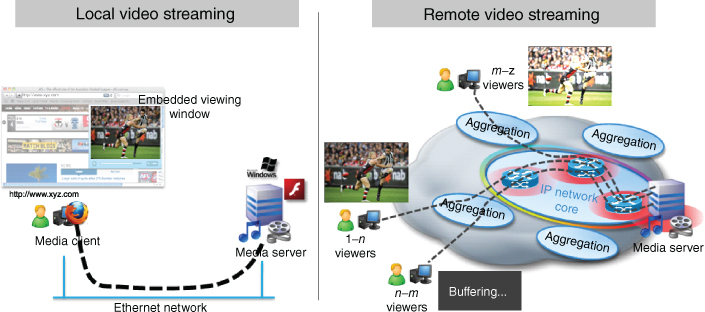
\includegraphics[resolution=120]{cdn-streaming.jpg}
		\caption{Optymalizacja strumieniowania wideo w sieciach CDN drugiej generacji. \cite{cdn}}
		\label{fig:cdn-streaming}
\end{figure}


Sieci rozproszone CDN są oparte o model chmury (np. Akamai Intelligent Platform). Dzięki sieciom CDN strony internetowe takie jak Facebook czy Twitter (klienci Akamai), pomimo że gromadzą dane z całego świata, mogą działać w czasie rzeczywistym. \cite{ccCambridge}

Za sprawą rosnącego znaczenia \textbf{Internetu Rzeczy}, przed technologiami w modelu chmury obliczeniowej stoją kolejne wyzwania. Internet Rzeczy znajduje użycie już teraz, czego dobrym przykładem są inteligentne zegarki. Wizja \textit{networked society} obejmuje jednak znacznie więcej, np. korzystanie z samoprowadzących się samochodów (rysunek \ref{fig:fog-samochod}) czy wspomaganie opieki zdrowotnej przez choćby automatyczne powiadomienie rodziny o zawale serca u pacjenta. Tego rodzaju usługi wymagają braku jakichkolwiek opóźnień. Ma to zostać zapewnione przez dodatkową warstwę, która podobnie jak CDN znajdowałaby się bliżej użytkownika niż centrum danych, ale potrafiłaby także wstępnie przetworzyć dane czy też zwrócić wynik bez angażowania do tego chmury.

\begin{figure}[h]
	\centering
			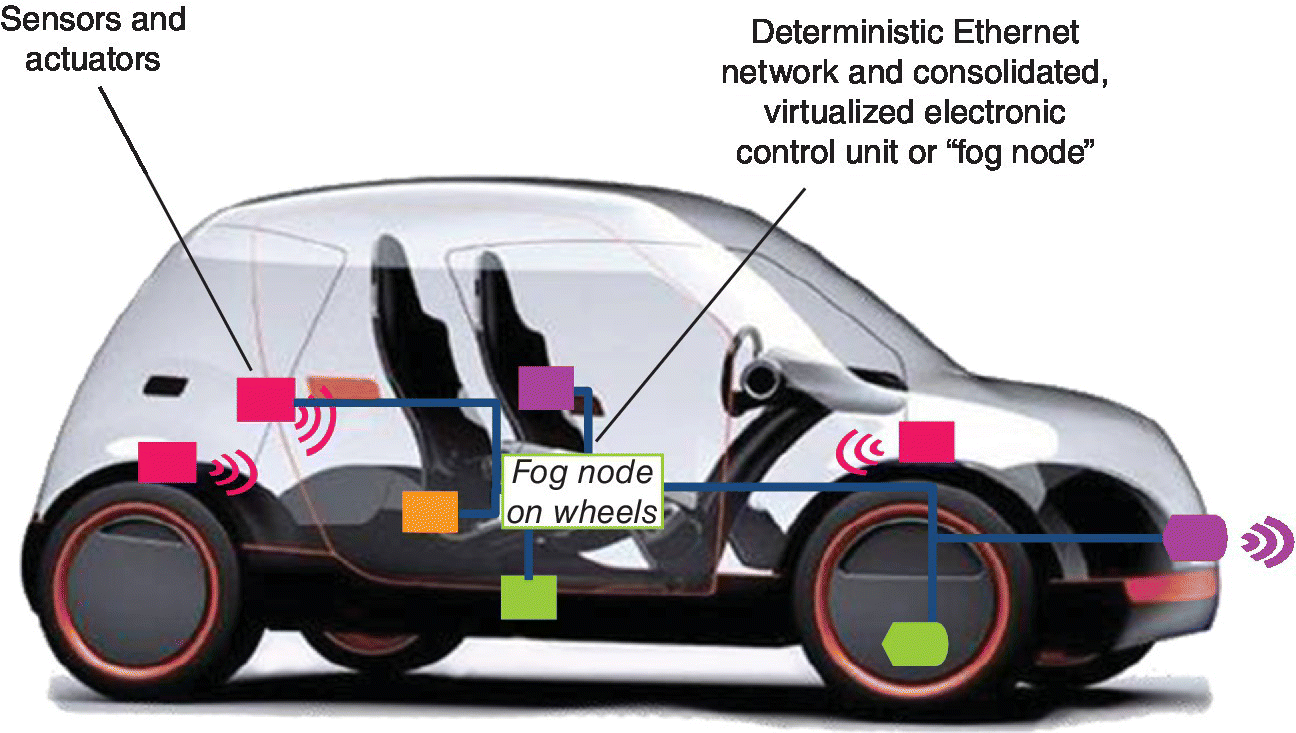
\includegraphics[width=0.5\textwidth]{fog-samochod.png}
		\caption{Zastosowanie Fog Computing w samoprowadzącym się samochodzie. \cite{fog5g}}
		\label{fig:fog-samochod}
\end{figure}

W 2012 r. firma Cisco przedstawiła koncepcję \textbf{Fog Computing} (,,mgły obliczeniowej''). Mgła ma stanowić warstwę pośredniczącą pomiędzy urządzeniami IoT a chmurą. Warstwa ta ma być ulokowana na routerze danego gospodarstwa domowego. Do zadań mgły należy wstępna obróbka danych, komunikacja z chmurą (już z użyciem mniejszej ilości danych), a także obsługa urządzeń IoT nawet jeśli w danym momencie brakuje połączenia z Internetem. Przykładowo, takie zadania jak rozpoznawanie obrazów mogą odbywać się już na etapie routera, bez konieczności przesyłania danych przez Internet. Konkretną propozycją Cisco było oprogramowanie Cisco IOx. \cite{fogArticle, iotArchitects}

Fog Computing nie stanowi jedynej koncepcji tego typu, jednakowoż brzmienie tej nazwy jest bardzo wyraziste i w literaturze wybija się na tle innych nazw. Być może z biegiem lat cała rodzina koncepcji przyspieszania technologii IoT będzie w ten sposób nazywana. Do innych koncepcji należą:
\begin{description}
\item [Cyber Foraging] Pojęcie przedstawione w 2001 r. w artykule M. Satyanarayanan'a. Technika polegająca na odciążaniu urządzeń mobilnych przez przekazanie wymagających obliczeniowo zadań do serwerów-surogatów i zwrócenie temu urządzeniu wyniku z niskim opóźnieniem. W przypadku braku serwera znajdującego się wystarczająco blisko, zadanie zostaje wykonane na miarę ograniczonych możliwości urządzenia mobilnego. \cite{fogArticle, fog5g}
\item [Cloudlet] Pojęcie przedstawione w 2009 r. w artykule współtworzonym przez Satyanarayanan'a. W odróżnieniu od Cyber Foragingu, cloudlety wykorzystują techniki wirtualizacji, co pozwala na ich skalowanie w zależności od wymagań użytkowników. Są to chmury znajdujące się bliżej użytkownika. Może to być np. chmura prywatna używana w przedsiębiorstwie. Nie ma wymogów, aby cloudlety komunikowały się dalej z chmurą publiczną. \cite{fogArticle, fog5g}
\item [Multi-Access Edge Computing (MEC)] Koncepcja pierwotnie nazwana ,,Mobile Edge Computing'' przez Europejski Instytut Norm Telekomunikacyjnych, gdyż była wiązana z telefonią komórkową oraz siecią radiową, lecz w 2017 r. została rozszerzona do wszystkich sieci. W tej koncepcji kładzie się nacisk na odciążanie chmur przez wykonywanie niektórych usług na krawędzi sieci \textit{(edge)}, tj. w pobliżu bramy sieciowej na różnych poziomach. Istotny element tej koncepcji stanowi upowszechnienie superszybkiej sieci 5G. \cite{fogArticle, fog5g}
\end{description}

Obecnie można zaobserwować rozwój zarówno w kierunku Fog Computingu jak i Edge Computingu:
\begin{itemize}
\item W 2015 r. powstało OpenFog Consortium. W 2017 r. konsorcjum opublikowało dokument referencyjny definiujący architekturę dla systemu w modelu Fog Computing. \cite{fogArticle, iotArchitects}
\item W 2017 r. powstało oprogramowanie ParaDrop, otwartoźródłowe oprogramowanie dla routerów w modelu Fog Computing. \cite{fog5g}
\item Główni dostawcy usług chmurowych udostępnili usługi typu \textit{edge}: AWS Lambda@Edge (lipiec 2017) \cite{siteAmazonLambdaEdge}, Azure IoT Edge (czerwiec 2018 r.) \cite{siteAzureIotEdge}, Google Cloud IoT Edge (wersja alpha, czerwiec 2018 r.)\cite{siteGoogleIotEdge}. 
\end{itemize}



\section{Wymagania stawiane współczesnym chmurom}

Powszechnie korzysta się z atrybutów określonych przez amerykański Narodowy Instytut Standaryzacji i Technologii w 2011 r., zwanych \textbf{modelem NIST}. Wyróżnia on cechy zasadnicze, modele dostarczania usług i formy wdrożenia. \cite{nistArticle, ccCambridge, azurePackt}

\subsection{Zasadnicze cechy chmury}

Do cech zasadniczych należą:

\begin{description}
\item [Samoobsługa] Aby skorzystać z usługi w chmurze czy zmodyfikować jej zakres, nie jest konieczna interwencja pracownika usługodawcy. Do samoobsługi służy panel administracyjny udostępniony przez usługodawcę.
\item [Szeroki dostęp przez sieć] Chmura powinna umożliwiać użytkownikom łączenie się przez sieć bez względu na to gdzie się znajdują i kiedy chcą skorzystać z usługi.
\item [Pula zasobów] Zasoby takie jak moc procesora, dyski, pamięć, mają być widoczne jako zasoby wirtualne oraz posiadać właściwość \textit{multi-tenancy} (z jednego zasobu może korzystać wiele niezależnych osób, nie mając na to wpływu i nie wiedząc o tym).
\item [Wysoka elastyczność] Dostępność zasobów ma być dozowana tak by dla użytkownika wyglądało to na nieskończoną ilość.
\item [Zliczanie zużycia] Dla każdego użytkownika stosowany jest mechanizm zliczania jego rzeczywistego zużycia danych usług. Zużycie jest transparentne dla obu stron, m.in. przez udostępnienie stosownych paneli służących do monitorowania i raportowania.
\end{description}

\subsection{Modele dostarczania usług}

Co do zasady istnieją 3 modele dostarczania usług:
\begin{itemize}
\item IaaS -- Infrastruktura jako usługa (ang. \textit{Infrastructure as a Service}),
\item PaaS -- Platforma jako usługa (ang. \textit{Platform as a Service)},
\item SaaS -- Oprogramowanie jako usługa (ang. \textit{Software as a Service}).
\end{itemize}
W literaturze i innych publikacjach często można spotkać się także z innymi podobnymi zwrotami w formie \textit{,,... as a Service''}, jednak zawsze jest to podkategoria dla tych powyższych. IaaS, PaaS i SaaS stanowią następujące po sobie warstwy. W przypadku wątpliwości związanej z klasyfikacją danej usługi wszelkie wątpliwości rozwiewa schemat umieszczony na rysunku \ref{fig:iaas-paas-saas}.

\begin{figure}[h]
	\centering
			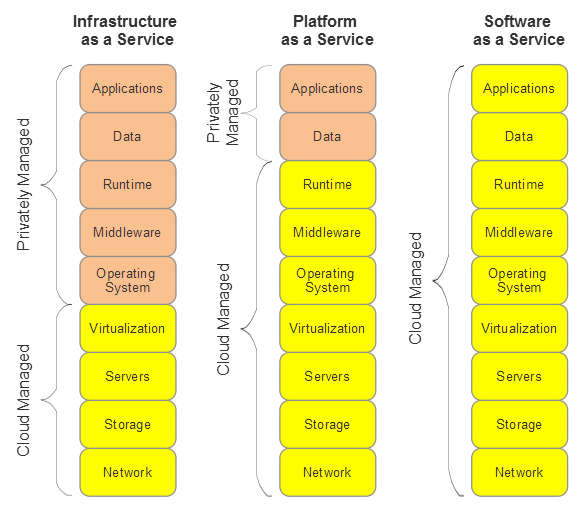
\includegraphics[width=0.7\textwidth]{iaas-paas-saas.png}
		\caption{Odpowiedzialność dostawcy usług chmurowych przy różnych ich rodzajach \cite{iotArchitects}}
		\label{fig:iaas-paas-saas}
\end{figure}

\textbf{IaaS} to wirtualne zasoby udostępnione jako usługa. Ponieważ wirtualizacja zasobów stanowi podstawową technikę stosowaną w modelu chmury, IaaS występuje zawsze gdy są udostępniane np. serwery wirtualne, dyski w chmurze czy sieci wirtualne. Przykładowe podgrupy to:
\begin{itemize}
\item NaaS (\textit{Network} -- sieć) -- sieci wirtualne,
\item CaaS (\textit{Container} -- kontener) -- usługa konteneryzacji,
\item KaaS (Kubernetes) -- CaaS z wykorzystaniem Kubernetes.
\end{itemize}
Klasyfikacja usługi CaaS może uchodzić za niejednoznaczną, ponieważ IaaS kojarzy się głównie z serwerami wirtualnymi, a kontenery z tworzeniem aplikacji. Podobnie jak serwery wirtualne odpowiadają wirtualizacji z użyciem nadzorcy typu 1, tak kontenery odpowiadają wirtualizacji na poziomie systemu operacyjnego. Stąd usługi, w których zarządzanie kontenerami jest wyeksponowane dla użytkownika, można zaliczyć do grupy IaaS.

W \textbf{PaaS} jako platformę określa się każde oprogramowanie umożliwiające użytkownikowi (programiście) zarządzanie jego własnymi aplikacjami. Warstwa ta jest zawsze zbudowana na IaaS, gdyż owo oprogramowanie musi działać na jakimś systemie operacyjnym na maszynie wirtualnej. Warstwa PaaS obejmuje wszystko co jest potrzebne programiście, by jego aplikacja mogła działać w chmurze: wsparcie dla różnych języków programowania, systemy bazodanowe, serwer WWW. Przykładowe podgrupy to:
\begin{itemize}
\item FaaS (\textit{Functions} -- funkcje) -- wdrażanie w modelu serverless,
\item DBaaS (\textit{Database} -- baza danych) -- usługa dzięki której nie trzeba samemu instalować bazy danych ani nią administrować,
\item BaaS/MBaaS (\textit{Mobile Backend}) -- wspomaganie aplikacji użytkownika narzędziami służącymi np. do wysyłania notyfikacji na urządzenia mobilne.
\end{itemize}

Warstwa \textbf{SaaS} obejmuje gotowe do użycia aplikacje. Na tej warstwie cała aplikacja znajduje się pod kontrolą dostawcy usługi, użytkownik może ją jedynie skonfigurować. Jest to najbardziej dojrzały model dostarczania usługi chmurowej, był stosowany już w 1999 r. przez Salesforce. Do rozwiązań SaaS należą m.in. popularne aplikacje dostępne przez przeglądarkę internetową: Gmail, Dropbox, Microsoft Office 365. Przykładowe podgrupy to:
\begin{itemize}
\item DaaS (\textit{Data} -- dane) -- usługa dostępu do danych zebranych np. przez Visa czy MasterCard aby pomóc personalizować przekaz reklamowy,
\item SECaaS (\textit{Security} -- bezpieczeństwo) -- narzędzia wspierające bezpieczeństwo, np. programy antywirusowe.
\end{itemize}

\subsection{Formy wdrożenia}

Istnieją 4 formy wdrożenia, zależne od zakładanej ilości użytkowników chmury:

\begin{description}
\item [Chmura prywatna] Jest to chmura stworzona na potrzeby danej organizacji, bez możliwości dostępu z zewnątrz. Fizyczne serwery tworzące chmurę mogą znajdować się wewnątrz sieci lokalnej organizacji (typ \textit{on-premises}) bądź poza siecią lokalną, ale wciąż pod pełną kontrolą tej organizacji (typ \textit{off-premises}), np. w wynajmowanej serwerowni. Ponieważ każdy kto ma dostęp do chmury jest ze sobą powiązany, nie występuje właściwość \textit{multi-tenancy} prowadząca do optymalizacji kosztów.
\item [Chmura społecznościowa] Chmura dostępna dla wielu organizacji, które łączy wspólna misja czy cel, a zamknięta dla wszystkich spoza społeczności. Może być zarządzana przez jedną bądź wiele organizacji należących do społeczności. Podobnie jak chmura prywatna, może być \textit{on-premises} bądź \textit{off-premises}.
\item [Chmura publiczna] Chmura dostępna dla wszystkich, dostępna tylko przez sieć publiczną. Nie ma możliwości stworzenia chmury publicznej typu \textit{on-premises}. Posiada właściwość \textit{multi-tenancy}. Zarządzanie odbywa się w pełni po stronie usługodawcy.
\item [Chmura hybrydowa] Połączenie chmury prywatnej bądź społecznościowej oraz chmury publicznej. Taki układ pozwala np. na obsługę standardowego ruchu za pomocą chmury prywatnej, a w przypadku wzmożonego obciążenia (godziny wieczorne, wybrany dzień w roku) przekierowanie części ruchu na chmurę publiczną.
\end{description}

\section{Dokąd zmierza rozwój Cloud Computingu}

Na podstawie historii najnowszej, a także mając na uwadze cele jakie stawia sobie technologia, autorka pracy dostrzega następujące kierunki rozwoju:
\begin{itemize}
\item \textbf{Dążenie do eliminacji problemu \textit{vendor lock-in}} (uzależnienia technologicznego od wybranego dostawcy usług chmurowych) \\
Natychmiastowa popularność konteneryzacji, Kubernetes jako usługa oraz pomysły takie jak Kubeless i Serverless Framework pozwalają wnioskować, że dalsza ewolucja dąży do wypracowania uniwersalnych standardów wytwarzania aplikacji dla chmury.

\item \textbf{Unifikacja systemów baz danych} \\
W ostatnich latach stworzono wiele innowacyjnych systemów baz danych. Ilość wariantów do wybrania stała się wręcz przytłaczająca. Dla jednego projektu może być potrzebne nawet kilka typów baz, dodatkowo nawet w ramach jednego typu są różne możliwości. Microsoft dostrzegł ten problem i stworzył usługę Azure CosmosDB, obsługującą wiele typów baz. Zdaniem autorki to nie jest ostatnie słowo wypowiedziane w tym kierunku. System pozbawiony problemu vendor lock-in, sam dobierający format przechowywania danych, byłby wielkim ułatwieniem dla programistów.

\item \textbf{Usprawnienie modelu serverless} \\
Usługa AWS Lambda powstała w 2014 r., a Google Cloud Functions wyszła z fazy poglądowej dopiero miesiąc temu. Według autorki w przypadku usług FaaS konkurencja istnieje na tyle krótko, że dostarczyciele usług mogą się jeszcze wiele od siebie nawzajem nauczyć i zastosować nowe pomysły, które nieco zmienią implementacje tego typu usług. 

\item \textbf{Wdrażanie Edge Computingu i Fog Computingu} \\
Pomimo że chmura stanowi podstawę dla Internetu Rzeczy, dobrze rozwinięta ,,warstwa pośrednia'' jest niezbędna by tworzyć inteligentne miasta. Autorka spodziewa się większego zainteresowania koncepcją Edge, ponieważ nie wymaga aktualizacji routerów u użytkowników, więc cały proces dla użytkowników mógłby przebiegać przezroczyście. Router typu Fog mógłby znajdować się w gotowym nowoczesnym produkcie, np. w samoprowadzącym się samochodzie. 

\item \textbf{Dążenie do uproszczenia wdrażania kontenerów w chmurze} \\
Usługi typu CaaS były pierwszym krokiem do uproszczenia zarządzania kontenerami. Oferują przyjazne panele administracyjne, niewymagające korzystania z CLI. Pod koniec 2017 r. pojawił się nowy trend polegający na możliwości wdrażania kontenerów w chmurze bez konieczności zarządzania orkiestratorem oraz maszynami wirtualnymi. Amazon udostępnił AWS Fargate w listopadzie 2017 r.,\cite{siteAwsFargateIntroducing} a Microsoft udostępnił Web App for Containers we wrześniu 2017 r.\cite{siteAzureWebAppContainersAvailable} oraz Azure Container Instances w kwietniu 2018 r.\cite{siteAzureContainerInstancesIntroducing} Google nie posiada jeszcze swojego rozwiązania tego typu. Można zatem spodziewać się odpowiedzi ze strony Google oraz dopracowania tego typu rozwiązań w taki sposób, aby przeciętnemu programiście wiedza o konfiguracji Kubernetes nie była potrzebna w codziennej pracy.

\end{itemize}

%\begin{figure}[h]
%	\centering
%			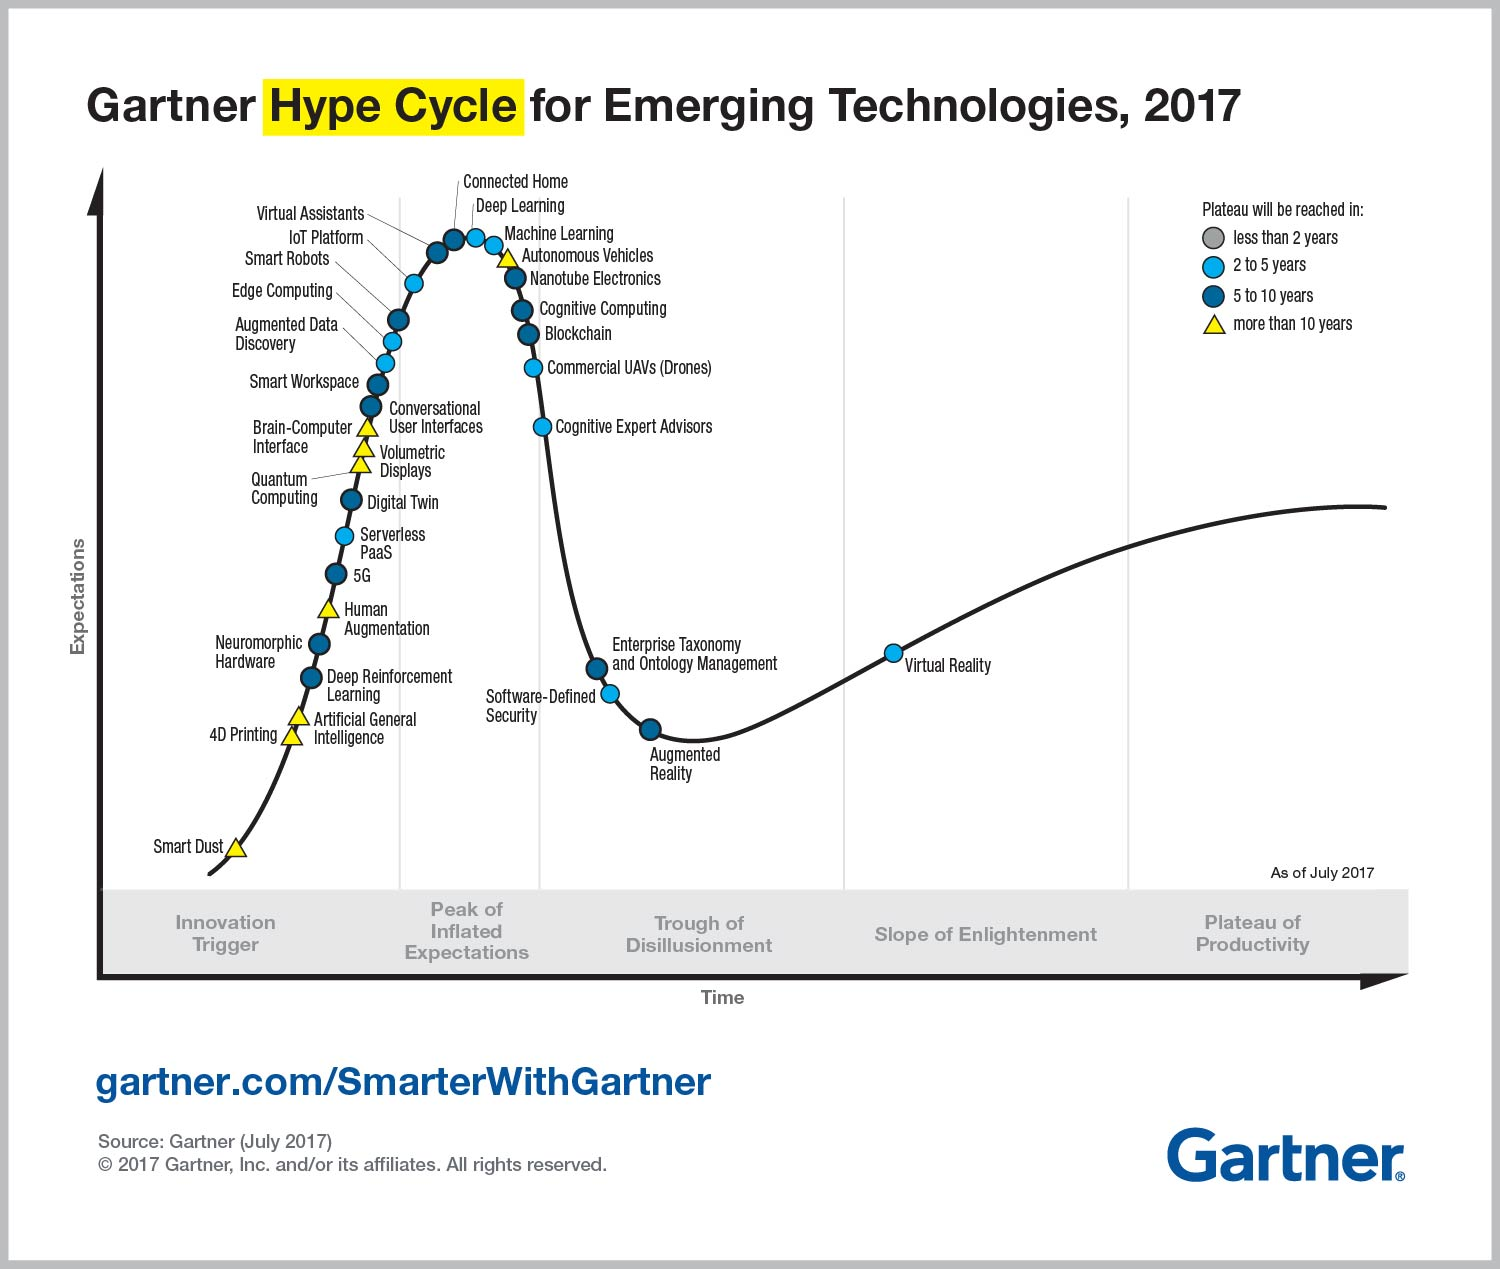
\includegraphics[width=\textwidth]{gartner-trends.jpg}
%		\caption{Raport dot. technologicznych trendów wykonany przez firmę Gartner w sierpniu 2017 r. \cite{siteGartnerTrends}}
%		\label{fig:gartner-trends}
%\end{figure}


%\begin{figure}[h]
%	\centering
%			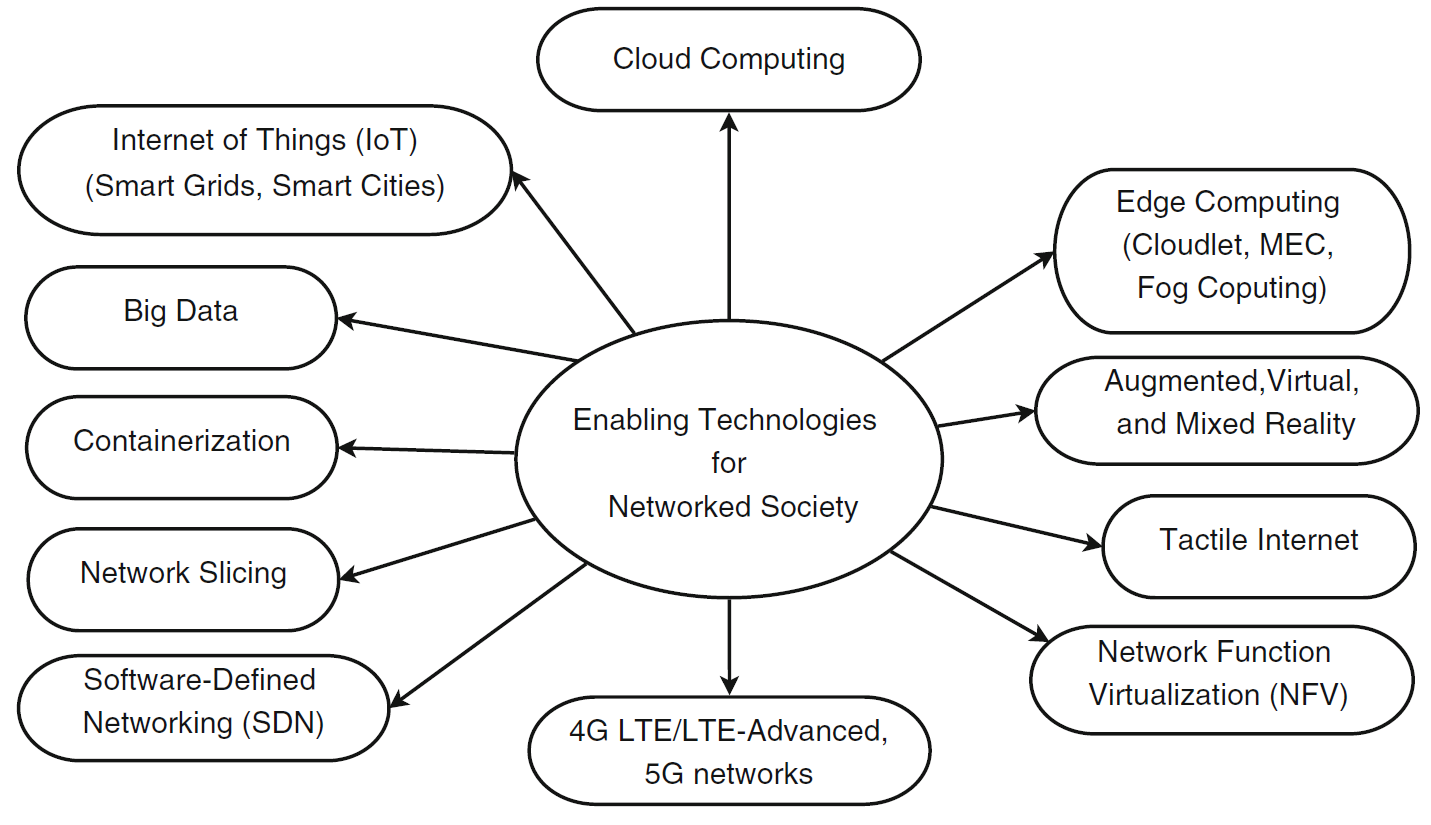
\includegraphics[width=\textwidth]{networked-society.png}
%		\caption{Technologie umożliwiające \textit{network society} \cite{ccSpringer}}
%		\label{fig:networked-society}
%\end{figure}



\chapter{Porównanie różnych podejść}

Usługę wspierającą urządzenie mobilne w chmurze można stworzyć i udostępnić na wiele sposobów. Dla programisty, który nie korzysta z chmury na co dzień, wybór ten może okazać się zaskakująco szeroki.

W niniejszym rozdziale zostaną przedstawione i porównane konkretne sposoby tworzenia usługi w chmurze, w kolejności od najstarszych do najnowszych rozwiązań.

Ze względu na największą popularność (rysunek \ref{fig:popularnosc}) oraz ilość dostępnych materiałów, w niniejszej pracy omawiając konkretne usługi chmurowe, koncentrowano się na chmurach AWS, Azure oraz Google Cloud.

\begin{figure}[h]
	\centering
			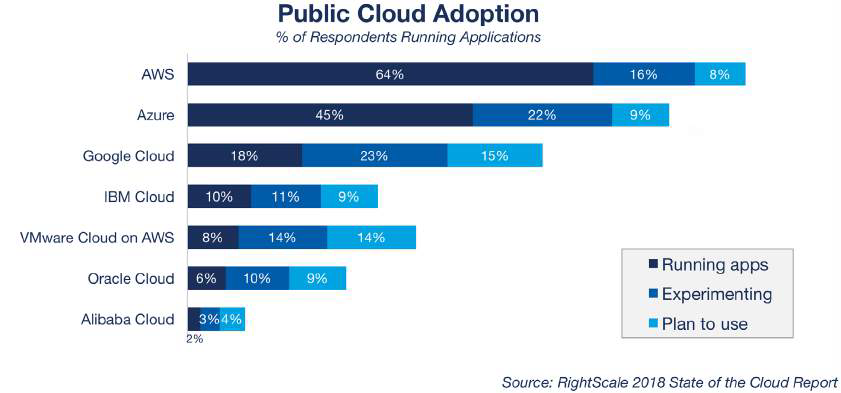
\includegraphics[width=\textwidth]{popularnosc.png}
		\caption{Popularność dostawców usług chmurowych \cite{rightscaleReport}}
		\label{fig:popularnosc}
\end{figure}

\section{Budowanie własnej chmury prywatnej} \label{section:chmuraPrywatna}

Jest to rozwiązanie polegające na budowaniu wszystkiego samemu u podstaw. Potrzebny jest przynajmniej jeden serwer, połączenie z Internetem oraz zespół osób dbających o infrastrukturę. Trzeba pamiętać nie tylko o standardowym przygotowaniu (odpowiednia temperatura pomieszczenia itp.), ale także o bieżących naprawach, konserwacji sprzętu, byciu na bieżąco z najnowszymi wymogami bezpieczeństwa. 

Pod względem idei posiadania własnych serwerów, chmura różni się tym, że docelowo zależy nam na korzyściach wynikających z dobrego skalowania systemów. Im więcej serwerów jest potrzebne, tym większym wyzwaniem staje się utrzymywanie całej infrastruktury i bycie odpowiedzialnym za jej bezpieczeństwo. 

\subsection*{Podsumowanie}

\subsubsection*{Główne narzędzia}
\begin{itemize}
\item hardware, łącze internetowe, prąd
\item system operacyjny dla serwera, np. CentOS, Debian, Windows Server
\item nadzorca typu 1 (ang. \textit{bare-metal hypervisor}), np. Xen, Oracle VM, Microsoft Hyper-V, VMware ESXi
\item dla usług IaaS: OpenStack, OpenNebula
\item dla usług CaaS: Kubernetes, Docker Swarm, Mezosphere DC/OS
\item dla usług PaaS: Cloud Foundry, OpenShift
\end{itemize}

\subsubsection{Perspektywy}
\begin{itemize}
\item Pełna niezależność.
\item Jedyna opcja dla organizacji, które muszą działać w obrębie sieci lokalnej, bez dostępu do Internetu (np. podczas ćwiczeń wojskowych).
\item Brak zmartwienia związanego z brakiem wiedzy o tym, gdzie fizycznie znajdują się dane.
\end{itemize}

\subsubsection{Ograniczenia}
\begin{itemize}
\item Konieczność samodzielnego troszczenia się o infrastrukturę: serwis komputerów, temperatura w serwerowni, czekanie na kuriera z nowymi częściami itp.
\item Konieczność samodzielnego aktualizowania oprogramowania i dbałości o bezpieczeństwo danych.
\item Brak możliwości skorzystania z ekonomii skali, obserwowanej w chmurach publicznych.
\end{itemize}

\section{Łączenie chmury prywatnej z chmurą hybrydową}

Posiadając chmurę prywatną, w przypadku skalowania w górę nie trzeba koniecznie kupować nowych serwerów. Można skonfigurować chmurę hybrydową, łącząc chmurę prywatną z publiczną. Chmury publiczne zazwyczaj udostępniają interfejs do łączenia ich przez VPN z chmurą prywatną.

Istnieje także możliwość pokuszenia się o zakup gotowego zestawu dostosowanego do tworzenia chmury hybrydowej, ze wsparciem firm specjalizujących się w tych rozwiązaniach.

Zgodnie z raportem RightScale 2018\cite{rightscaleReport}, z rozwiązań hybrydowych w 2017 r. korzystało 58\% ankietowanych, a rok później liczba ta spadła do 51\%. Jednocześnie odnotowano nadanie większego priorytetu chmurom publicznym (zwiększenie z 29\% do 38\%), a mniejszego hybrydowym (spadek z 50\% do 45\%).


\subsection*{Podsumowanie}



\subsubsection*{Główne usługi chmurowe}
Usługi przydatne przy tworzeniu chmury hybrydowej wymieniono w tabeli \ref{table:hybrid}.


\noindent
\begin{small}
\begin{table}[h!]
\newcolumntype{L}{>{\raggedright\arraybackslash}X}%
\begin{tabularx}{\textwidth}{ |L|L|L|L| }

\hline
\multirow{2}{*}{Typ usługi} & \multicolumn{3}{|c|}{Dostawca} \\

\cline{2-4}
& \multicolumn{1}{|c|}{AWS} & \multicolumn{1}{|c|}{GCP} & \multicolumn{1}{|c|}{Azure} \\

\hline
wirtualna prywatna sieć & Virtual Private Cloud & Virtual Private Cloud & Virtual Network \\
\hline
dedykowane prywatne połączenie & Direct Connect & Cloud Interconnect & Azure Express Route \\
\hline
zarządzanie kontami użytkowników & Identity and Access Management & Cloud Identity & Azure Active Directory \\
\hline
wsparcie bezpieczeństwa chmury prywatnej & Inspector & b/d & Azure Security Center \\
\hline
integracja danych & Storage Gateway & b/d & StorSimple \\
\hline 

\end{tabularx}


\caption{Główne interfejsy chmur publicznych dla chmur hybrydowych}
		\label{table:hybrid}

\end{table}
\end{small}

\subsubsection*{Gotowe zestawy do tworzenia chmur hybrydowych}
Gotowe zestawy integrujące dedykowany zestaw fizycznych urządzeń z wybraną chmurą publiczną wymieniono w tabeli \ref{table:hybridIntegrated}.

\noindent
\begin{small}
\begin{table}[h!]
\newcolumntype{L}{>{\raggedright\arraybackslash}X}%
\begin{tabularx}{\textwidth}{ |L|L|L| }

\hline
Nazwa & Chmura publiczna & Zestawy \\
\hline
Azure Stack \cite{siteAzureStack} & Microsoft Azure & 
Avanade Solution, \newline
Cisco Integrated System, \newline
Dell EMC Cloud, \newline
HPE ProLiant (HP), \newline
Huawei Hybrid Cloud Solution, \newline
Lenovo ThinkAgile SX, \newline
TERRA (Wortmann AG, Intel, and Microsoft) \\
\hline
Cisco and Google Cloud \cite{siteGoogleCisco} & Google Cloud & Cisco Hybrid Cloud Platform for Google Cloud \\
\hline


\end{tabularx}


\caption{Gotowe rozwiązania dla chmur hybrydowych}
		\label{table:hybridIntegrated}

\end{table}
\end{small}


\subsubsection{Perspektywy}
\begin{itemize}
\item Największa elastyczność -- korzystanie z zalet chmur prywatnych i publicznych.
\item Możliwość wykorzystywania chmury publicznej tylko w przypadku gdy prywatna infrastruktura przestaje wystarczać.
\item Możliwość tworzenia kopii zapasowej do chmury.
\item Możliwość wykorzystywania wybranych specjalistycznych zastosowań chmury publicznej.
\end{itemize}

\subsubsection{Ograniczenia}
\begin{itemize}
\item Konieczność utrzymywania rozwiązań zarówno chmury prywatnej jak i chmury publicznej.
\item Spowolnienie rozwoju przez zachowywanie kompatybilności pomiędzy chmurami.
\end{itemize}


\section{Wykupienie serwera wirtualnego w chmurze}\label{section:podejscieVm}

Jest to podejście, w którym rezygnuje się z zarządzania fizyczną infrastrukturą komputerową. Odchodzą zatem ograniczenia spotykane przy budowaniu własnej chmury prywatnej (opisane w sekcji  \ref{section:chmuraPrywatna}). Nadal jednak trzeba samodzielnie wybrać system operacyjny oraz doinstalować odpowiednie środowiska.

Serwer wirtualny w chmurze można łatwo pomylić ze zwykłym VPS (ang. \textit{Virtual Private Server}) oferowanym przez firmy hostingowe. Hosting VPS istniał również w czasach ,,przed'' Amazon EC2. Typowo polegał na podzieleniu zasobów jednej fizycznej maszyny na kilka mniejszych -- wirtualnych, za pomocą oprogramowania typu Xen. Podobnie jak fizyczny serwer, VPS miał odgórnie ustaloną ilość RAM, wielkość dysku twardego i limity CPU. Można postrzegać VPS jako tańszą alternatywę dla fizycznego serwera. 

Natomiast podejście ,,chmurowe'' do serwerów wirtualnych różni się od tradycyjnego podejścia VPS w następujących względach:
\begin{itemize}
\item Dochodzi warstwa abstrakcji, dzięki której maszyna wirtualna nie jest ściśle przypisana do fizycznej maszyny. Można zmieniać ilość przydzielonych zasobów oraz zmieniać ilość wirtualnych maszyn hostujących aplikację.
\item Rozliczanie odbywa się w modelu płatności za zużycie (\textit{utility computing}). Płatność za tradycyjne serwery wirtualne odbywa się w formie abonamentu, np. w przypadku miesięcznego okresu rozliczeniowego, chcąc używać VPS przez kilka dni, nadal należałoby zapłacić za cały miesiąc.
\item Zgodnie z modelem chmury NIST, panuje samoobsługa realizowana przy pomocy panelu administracyjnego. Nie ma konieczności składania zamówienia czy czekania na personel aż uruchomi skonfigurowaną maszynę.
\item Możliwość wykonania kopii zapasowej maszyny wirtualnej, znacznie ułatwione przez chmurową warstwę abstrakcji. 
\end{itemize}

W związku z dostępnością narzędzi przygotowanych do tworzenia chmur prywatnych, dostarczyciele serwerów VPS zaczęli stosować niektóre bądź wszystkie techniki wymienione powyżej. Wówczas główną różnicę stanowi zaplecze zasobów. W przypadku dużych chmur publicznych jest ono tak duże, że dla skalowania ilości maszyn wirtualnych w górę tworzy się iluzja nieskończoności zasobów, gdyż można zażyczyć sobie nawet dziesiątki tysięcy instancji serwerów wirtualnych. Dla mniejszych dostawców to wciąż może być zbyt wielkie wyzwanie.

Jednocześnie chmury publiczne nie stronią od świadczenia usług bardziej przypominających VPS. Spośród opcji rozliczania można wybrać takie uwzględniające rezerwację określonej puli zasobów na określony czas. Również istnieją możliwości wynajęcia serwera fizycznie odizolowanego od innych, np. w usłudze Amazon EC2 Dedicated Hosts.

Wynajmując prawdziwy serwer wirtualny w chmurze należy pamiętać, że to nie jest hosting, nawet jeśli go przypomina. Cechami chmury są skalowalność i płatność za zużycie. Podczas konfiguracji usługi IaaS istnieje możliwość indywidualnego doboru wielu parametrów, które należy dopasować w sposób optymalizujący koszty. W koszta należy również uwzględnić dodatkowe usługi poza maszynami wirtualnymi, np. wynajęcie przestrzeni dyskowej na kopie zapasowe maszyn wirtualnych, usługi typu Load Balancer, itp.

Do tworzenia maszyn wirtualnych można używać napisanych przez siebie programów wykorzystujące API usługodawcy. Dla popularnych technologii (Java, Python itp.) są dostępne SDK do obługi wybranej chmury, a także biblioteki obsługujące usługi IaaS wielu dostawców.

\subsection*{Podsumowanie}


\subsubsection*{Serwery wirtualne w chmurach publicznych}
\begin{itemize}
\item \textbf{Amazon Elastic Compute Cloud (EC2)} -- Aby uruchomić nową instancję, należy wybrać obraz AMI (ang. \textit{Amazon Machine Image}) zawierający system operacyjny wraz z oprogramowaniem, a także wybrać typ instancji zawierający wstępną konfigurację. Wraz z maszyną zostaje utworzony wirtualny dysk w usłudze Amazon Elastic Block Store. Można zmodyfikować domyślną konfigurację o dodanie m.in. load balancerów (Elastic Load Balancing), automatycznie skalującej się grupy (Amazon EC2 Auto Scaling), dodatkowych dysków w EBS. Wszystkie te usługi zostały zebrane wewnątrz panelu administracyjnego usługi EC2.
\item \textbf{Azure Virtual Machines} -- Wbrew mitom pozwala na utworzenie maszyn wirtualnych działających na systemach innych niż Windows, m.in. Ubuntu, Red Hat, SUSE, CoreOS, FreeBSD. Obrazy tych systemów znajdują się w Azure MarketPlace. Do skalowania służą Virtual Machine Scale Sets. Ciekawą opcję stanowią Azure Extensions, czyli skrypty automatycznie uruchamiane po uruchomieniu maszyny wirtualnej. W przypadku maszyn działających na systemie Linux dostępna jest również opcja Cloud-init, gdzie można zdefiniować listę paczek do doinstalowania po pierwszym uruchomieniu systemu. 
\item \textbf{Google Cloud Platform} -- Usługę Google wyróżnia prosty, schludny interfejs użytkownika. Do uruchomienia instancji maszyny wirtualnej z domyślnymi ustawieniami wystarcza jeden ekran z opcjami. W przypadku braku maszyn wirtualnych portal proponuje wykonać jeden projekt szacowany na 15 minut przy użyciu samouczka.
\end{itemize}

\subsubsection{Biblioteki przystosowane do obsługi wielu chmur IaaS}
\begin{itemize}
\item \textbf{Apache LibCloud} -- biblioteka dla języka Python. Obsługuje ponad 50 różnych dostawców.
\item \textbf{Apache jClouds} -- biblioteka dla języka Java. 
\item \textbf{Libretto} -- biblioteka dla języka Go.
\item \textbf{pkgcloud} -- biblioteka dla node.js.
\item \textbf{Fog} -- biblioteka dla Ruby.
\end{itemize}

\subsubsection{Perspektywy}
\begin{itemize}
\item Brak początkowej inwestycji w infrastrukturę.
\item Brak zmartwień związanych z samodzielnym administrowaniem serwerami.
\item Skalowalność infrastruktury.
\item Możliwość instalowania dowolnych środowisk.
\item Możliwość przeniesienia tradycyjnie napisanej aplikacji do chmury.
\end{itemize}

\subsubsection{Ograniczenia}
\begin{itemize}
\item Większy koszt w porównaniu z usługami PaaS (np. koszty licencji oprogramowania).
\item Konieczność samodzielnego administrowania oprogramowaniem.
\item Konieczność samodzielnego dbania o bezpieczeństwo i aktualizacje.
\item Skomplikowany model rozliczania -- mnogość parametrów od których zależy całkowity koszt usług. Niewystarczająca uwaga natychmiast odbija się na karcie podanej do rozliczeń. Autorka pracy ma w tym punkcie zastrzeżenie do firmy Amazon, ponieważ z jednej strony dużymi literami ogłasza możliwość darmowego przetestowania usług, a z drugiej strony samo założenie konta kosztuje 1 USD, a założenie maszyny wirtualnej (która sama w sobie była bezpłatna) z domyślnymi opcjami kosztowało kolejnego. 
\item Organizacje celujące w ograniczoną ilość odbiorców mogą potrzebować serwera wirtualnego, ale nie potrzebować skalowalności jaką daje chmura. Dla nich odległość do centrum danych mieszczącego się w innym kraju oraz korzystanie z oferty zagranicznych usługodawców mogą stanowić wady, a hosting typu VPS dostarczany z pobliskiej miejscowości lepszą alternatywę.
\end{itemize}

\section{Usługi typu PaaS oparte o maszyny wirtualne w chmurach publicznych}\label{section:podejsciePaas}

Jest to pierwsza generacja usług typu PaaS, gdzie w odróżnieniu od tworzenia własnej maszyny wirtualnej i na niej uruchamianiu aplikacji, twórca aplikacji ma skupić się jedynie na dostarczeniu aplikacji, a utworzenie odpowiednich maszyn wirtualnych znajduje się po stronie usługodawcy. Obecnie funkcjonują również inne sposoby usprawniające pracę programisty w kontekście usług chmurowych i te sposoby zostały omówione w kolejnych sekcjach.

Główną charakterystyką tych usług jest to, że są one specyficzne dla danej chmury. Każda posiada własne mechanizmy łączenia ze sobą różnych typów usług stworzonych dla developerów. Mogą różnić się m.in. wspieranymi technologiami. Przykładowo, firma Microsoft wspiera szerokie spektrum technologii, ale zawsze w pierwszej kolejności .NET Framework. Chmura Google zaczynała od wsparcia dla Javy i Pythona, a obecnie można tworzyć również w Node.js, PHP, Go, Ruby, .NET Core.

Wadą tego typu rozwiązań jest duże przywiązanie do wybranego dostawcy usług. Każdy udostępnia swój własny SDK dla wspieranych języków programowania i przeniesienie aplikacji napisanej w ten sposób do innego usługodawcy wymaga przepisywania znacznej części kodu lub może być niemożliwe.

Platformy aplikacji w chmurach publicznych są dobrze przygotowane do tworzenia aplikacji typu \textit{cloud native}, zgodnych z metodyką \textit{12-factor app}. Usługodawcy dbają również o łatwe stosowanie strategii DevOps na swoich platformach. Powyższe implikuje, iż tworząc tego typu aplikacje warto wcześniej dobrze zapoznać się z metodyką 12-factor, jak również z wzorcami projektowymi towarzyszącymi tworzeniu mikrousług. 

Wsparcie dla tworzenia aplikacji w chmurze może polegać na:
\begin{itemize}
\item budowaniu back-endu dla aplikacji mobilnych -- jest to zastosowanie, na którym koncentruje się niniejsza praca. Polega na udostępnianiu węzłów końcowych API (ang. \textit{endpoints}), z którymi komunikuje się aplikacja mobilna. Odbywa się to przy pomocy REST lub SOAP;
\item serwisie notyfikacji -- umożliwia wysyłanie notyfikacji push z poziomu chmury;
\item aplikacjach logicznych -- umożliwiają definiowanie przepływów, np. segregacja wiadomości z Twittera a następnie automatyczne wysłanie e-maili;
\item stronach internetowych -- gotowe szablony stron internetowych opartych np. o Wordpress czy Joomla!;
\item korelowaniu i analizie różnych źródeł danych.
\end{itemize}

\subsection*{Podsumowanie}

\subsubsection{Usługi służące tworzeniu aplikacji}
\begin{itemize}
\item \textbf{AWS Elastic Beanstalk} -- aplikacje internetowe oraz mikrousługi. Obsługiwane języki: Java, PHP, Python, Node.js, Ruby, .NET, Go
\item \textbf{Azure App Service}
	\begin{itemize}
		\item \textbf{Web Apps} -- aplikacje internetowe oraz mikrousługi. Obsługiwane języki:  Java, PHP, Python, Node.js, Ruby, .NET
		\item \textbf{Mobile Apps} -- tworzenie backendu dla aplikacji mobilnych, możliwość synchronizacji offline, połączenie z Notification Hubs do wysyłania notyfikacji push
		\item \textbf{WebJobs} -- zadania wykonywane po odebraniu zdarzenia
	\end{itemize}
\item \textbf{Google App Engine} -- platforma tworzenia mikrousług. Obsługiwane języki: Java, PHP, Python, Node.js, Ruby, .NET, Go
\item \textbf{Google Cloud Endpoints} -- narzędzia do generowania API i bibliotek na podstawie aplikacji w App Engine
\end{itemize}

\subsubsection{Główne usługi wspierające tworzenie back-endu dla aplikacji mobilnych}

AWS:
\begin{itemize}
\item \textbf{Simple Storage Services (S3)} -- przechowywanie danych binarnych
\item \textbf{Amazon DynamoDB} -- baza obsługująca dwa modele danych: dokumentowe oraz klucz-wartość
\item \textbf{Amazon Relational Database Service (RDS)} -- relacyjna baza danych kompatybilna z różnymi silnikami baz danych: PostgreSQL, MySQL, MariaDB, Oracle Database, Microsoft SQL Server
\item \textbf{Amazon Aurora} -- baza kompatybilna z PostgreSQL oraz MySQL, zarządzana przez RDS
\end{itemize}

\noindent
Azure:
\begin{itemize}
\item \textbf{Azure Storage}
	\begin{itemize}
		\item \textbf{Blob Storage} -- dane binarne
		\item \textbf{Table Storage} -- baza NoSQL typu \textit{wide-column}
		\item \textbf{Queue Storage} -- kolejki komunikatów
	\end{itemize}
\item \textbf{Azure Cosmos DB} -- baza NoSQL obsługująca wiele modeli danych: grafowe, dokumentowe, klucz-wartość oraz \textit{wide-column}
\item \textbf{Azure SQL Database} -- baza relacyjna kompatybilna z MS SQL
\item \textbf{Azure Notification Hubs} -- wysyłanie notyfikacji push na urządzenia z różnymi systemami operacyjnymi
\item \textbf{Azure Cognitive Services} -- usługi ułatwiające uczenie maszynowe, np. rozpoznawanie obrazów

\end{itemize}

\noindent
Google Cloud:
\begin{itemize}
\item \textbf{Google Cloud Datastore} -- baza NoSQL typu dokumentowego
\item \textbf{Google Cloud Firebase} -- baza NoSQL typu dokumentowego, będąca następcą Datastore; aktualnie w wersji beta
\item \textbf{Google Cloud SQL} -- baza relacyjna kompatybilna z MySQL
\item \textbf{Google Cloud Storage} -- przechowywanie danych binarnych
\item \textbf{Google Cloud Bigtable} -- baza typu \textit{wide-column}
\item \textbf{Google Cloud Spanner} -- baza relacyjna skalowalna horyzontalnie

\end{itemize}

\subsubsection{Perspektywy}
\begin{itemize}
\item Tańszy koszt w porównaniu z IaaS.
\item Koncentracja na zadaniu tworzenia aplikacji.
\item Dostęp do specjalistycznych usług, np. rozpoznawania obrazów.
\item Wsparcie dla DevOps w zintegrowanym środowisku danej platformy.
\end{itemize}

\subsubsection{Ograniczenia}
\begin{itemize}
\item Problem \textit{vendor lock-in} -- trudność w przenoszeniu aplikacji na inną platformę.
\item Konieczność zastosowania się do rozwiązań dyktowanych przez początkowo wybranego usługodawcę. Można napotkać na trudność we wprowadzaniu zmian do już istniejących aplikacji, ponieważ gdy usługodawca zmieni API, wprowadzając zmianę należy również dostosować aplikację do aktualnego API.
\item Wiązanie się z konkretnym usługodawcą oznacza konieczność zatrudniania programistów wyspecjalizowanych w usługach tego dostawcy. Występuje tu potencjalna trudność w znalezieniu pracownika oraz płaceniu za jego wąską specjalizację.
\item Mniejsza elastyczność niż w IaaS.
\item Konieczność zapoznania się z dobrymi praktykami tworzenia aplikacji \textit{cloud native} a także mikrousług.
\item Utrudnione rozwijanie aplikacji offline, bez dostępu do platformy.
\end{itemize}

\section{Samodzielna instalacja orkiestratora kontenerów}\label{section:instalujKontenery}

Jest to podejście, które do niedawna (do czasu publikacji usług typu CaaS) miało szczególne znaczenie, ponieważ pozwalało na korzystanie z Cloud Foundry czy Kubernetes pomimo braku specjalnego wsparcia po stronie chmur publicznych. 

Rozwiązania te dzięki wykorzystaniu kontenerów eliminują problem \textit{vendor lock-in}. Trzeba jednak samemu przejść przez proces instalacji odpowiedniego oprogramowania na serwerze wirtualnym lub fizycznej maszynie (ang. \textit{bare-metal}).

Chmury publiczne wspierają konteneryzację jako usługę od stosunkowo niedawna. Wciąż 57\% wdrożeń Kubernetes opiera się na Amazon EC2. Podejście oparte o samodzielną instalację niejednokrotnie będzie można spotkać w literaturze, na stronach internetowych oraz w już wdrożonych aplikacjach.

\subsection*{Podsumowanie}

Główne usługi chmurowe oraz zalety i wady dziedziczą się odpowiednio z wynajmu maszyny wirtualnej (sekcja \ref{section:podejscieVm}) bądź z tworzenia chmury prywatnej (sekcja \ref{section:chmuraPrywatna}).

\subsubsection{Główne narzędzia}
\begin{itemize}
\item Kubernetes
\item Docker Swarm
\item Mezosphere DC/OS
\item Cloud Foundry
\end{itemize}

\subsubsection{Perspektywy}
\begin{itemize}
\item Brak problemu \textit{vendor lock-in}.
\item Możliwość korzystania z obrazów Dockera, które uchodzą za standard obsługiwany na każdej platformie.
\item Możliwość skalowania aplikacji w standardowy sposób.
\item Możliwość korzystania z dowolnych technologii w odpowiednich wersjach.
\item Możliwość zatrudniania programistów o różnych umiejętnościach, ponieważ nie muszą znać technologii podyktowanych przez wybranego dostawcę usług chmurowych. Co więcej, każda mikrousługa może być napisana w innej technologii, więc łatwiej znaleźć odpowiednich specjalistów.
\item Możliwość rozwijania oprogramowania lokalnie na komputerze, mając pewność, że na środowisku produkcyjnym będą obowiązywały dokładnie te same narzędzia.
\end{itemize}

\subsubsection{Ograniczenia}
\begin{itemize}
\item Konieczność samodzielnej instalacji potrzebnego środowiska.
\end{itemize}

\section{Usługa konteneryzacji w chmurach publicznych}\label{section:caas}

Na fali ogromnej popularności Dockera, a później Kubernetes, zaczęły powstawać usługi typu CaaS/KaaS, pozwalające na korzystanie z dobrodziejstw orkiestratorów kontenerów bez konieczności ich instalowania. Usługi te zazwyczaj pozwalają zarządzać orkiestratorem z poziomu narzędzia CLI bądź przy pomocy graficznego interfejsu (rysunek \ref{fig:kubernetes-engine}).

Do zarządzania obrazami kontenerów usługodawcy proponują specjalne rejestry kontenerów.

\begin{figure}[h]
	\centering
			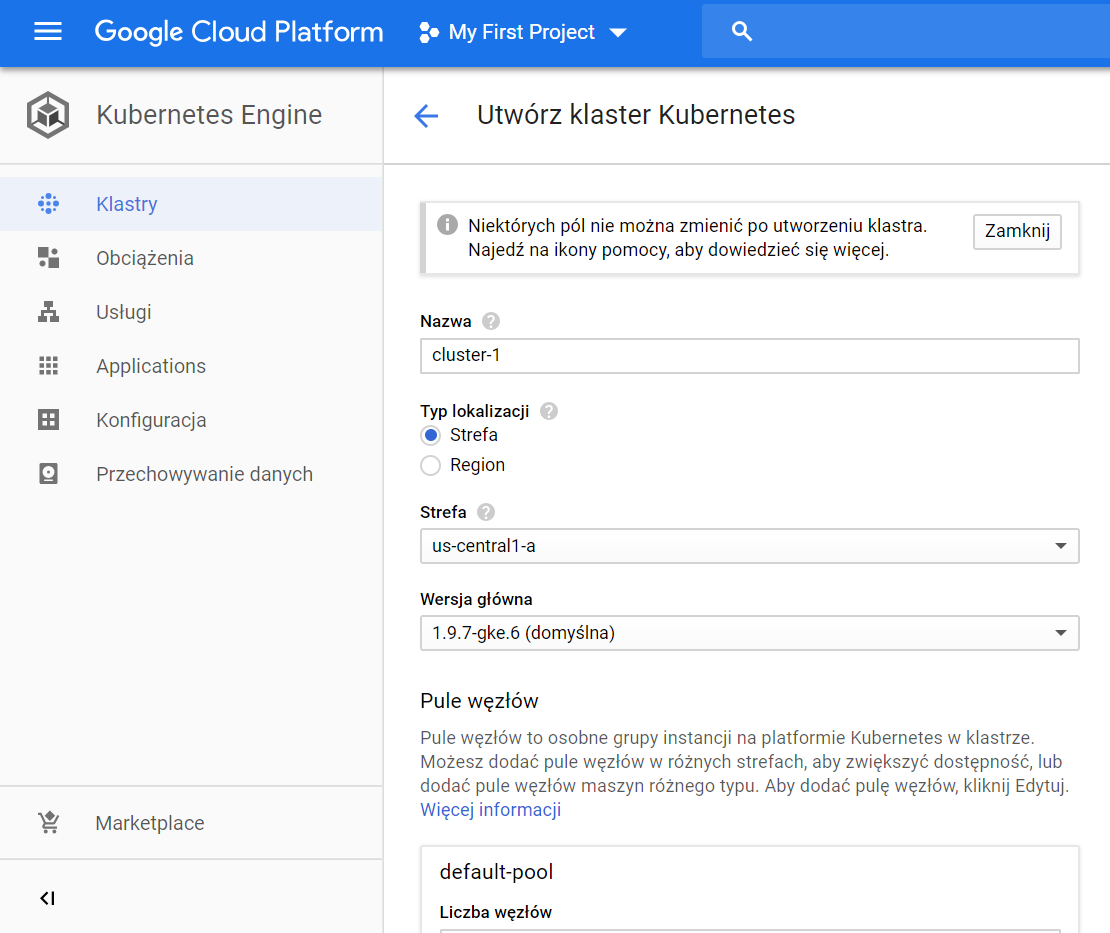
\includegraphics[width=\textwidth]{kubernetes-service.png}
		\caption{Graficzny interfejs pozwalający skonfigurować Kubernetes w Google Kubernetes Engine}
		\label{fig:kubernetes-engine}
\end{figure}

\subsection*{Podsumowanie}

\subsubsection{Usługi CaaS}

\begin{itemize}
\item \textbf{Google Kubernetes Engine}
\item \textbf{Azure Kubernetes Service (AKS)}
\item \textbf{Amazon ECS -- Amazon Elastic Container Service} -- własna implementacja orkiestracji kontenerów Dockera stworzona przez Amazona
\item \textbf{Amazon EKS -- Amazon Elastic Container Service for Kubernetes} -- wersja implementująca Kubernetes
\end{itemize}

\subsubsection{Usługi rejestru kontenerów}

\begin{itemize}
\item Amazon Elastic Container Registry
\item Azure Container Registry
\item Google Container Registry
\end{itemize}

\subsubsection{Perspektywy}

\begin{itemize}
\item Prosta możliwość wypróbowania i skorzystania z Kubernetes bez przechodzenia przez proces konfiguracji całej infrastruktury.
\item Główne zalety dziedziczą się z zalet opisanych w sekcji poświęconej samodzielnej instalacji orkiestratora kontenerów (sekcja \ref{section:instalujKontenery}).
\end{itemize}

\subsubsection{Ograniczenia}
\begin{itemize}
\item Konieczność zapoznania się z odpowiednim konfigurowaniem orkiestratora kontenerów. Jest to konfiguracja dotycząca infrastruktury, czyli dla twórcy aplikacji nie jest związana z programowaniem.
\item Pod względem tworzenia aplikacji wypada znać i umieć stosować w praktyce zasady dotyczące tworzenia aplikacji dla chmury, w szczególności mikrousług.
\end{itemize}


\section{Usługi typu PaaS oparte o kontenery w chmurach publicznych}

Aby na chmurze publicznej móc korzystać z kontenerów Dockera, nie trzeba koniecznie znać się na Kubernetes. Chmury publiczne wypracowały rozwiązania polegające na wdrożeniu w chmurze zadanego obrazu, bez konieczności konfigurowania infrastruktury na jakiej są uruchamiane.

Rozwiązania tego typu służą głównie w celu uruchomienia na chmurze pojedynczego kontenera. Jako inny przypadek użycia Azure podaje chaotyczne zapotrzebowanie (ang. \textit{traffic in spikes}, czyli ruch, który na wykresie wyglądałby jak kolce). Natomiast dla długo działających kontenerów ze stabilnym ruchem, Azure rekomenduje wykorzystanie CaaS. \cite{siteAzureContainerInstances}.

Podobnie jak w przypadku usług CaaS (sekcja \ref{section:caas}), do zarządzania obrazami kontenerów można użyć usługi rejestru kontenerów.

Opisywane podejście w czasie tworzenia pracy uchodzi za nowatorskie -- pierwsze rozwiązania tego typu pojawiły się pod koniec 2017 r., a firma Google póki do nie przedstawiła swojej propozycji.

\subsection*{Podsumowanie}

\subsubsection{Usługi instancji kontenerów}

\begin{itemize}
\item \textbf{AWS Fargate} -- usługi CaaS od Amazona, ECS i EKS, posiadają dwa tryby wdrożenia kontenera: tryb Fargate oraz tryb EC2. Fargate to możliwość wdrożenia kontenera bez konieczności zarządzania orkiestratorem i maszynami wirtualnymi. \cite{siteAwsFargate}
\item \textbf{AWS Elastic Beanstalk -- Deploying Elastic Beanstalk Applications from Docker Containers} -- opcja wdrażania aplikacji w Elastic Beanstalk za pomocą obrazu Dockera 
\item \textbf{Azure Container Instances} -- możliwość wdrażania instancji kontenerów rozliczana na podstawie sekund \cite{siteAzureContainerInstances}
\item \textbf{Azure App Service -- Web App for Containers} -- rozwinięcie App Service o możliwość wdrożenia obrazu kontenera.
\end{itemize}

\subsubsection{Usługi rejestru kontenerów}
Tak samo jak w sekcji dotyczącej usługi CaaS (sekcja \ref{section:caas}).

\subsubsection{Perspektywy}
\begin{itemize}
\item Niska bariera wejścia jeśli chodzi o wdrażanie obrazu kontenera do chmury publicznej.
\item Możliwość odroczenia nauki orkiestratora kontenerów do czasu wzrostu popularności aplikacji.
\item Główne zalety dziedziczą się z zalet opisanych w sekcji poświęconej samodzielnej instalacji orkiestratora kontenerów (sekcja \ref{section:instalujKontenery}).
\end{itemize}

\subsubsection{Ograniczenia}
\begin{itemize}
\item Podejście nie rozwiązuje całkowicie problemu nauki orkiestratora kontenerów.
\item Pod względem tworzenia aplikacji wypada znać i umieć stosować w praktyce zasady dotyczące tworzenia aplikacji dla chmury, w szczególności mikrousług.
\item Usługi tego typu są bardzo nowe, co może powodować zwiększone ryzyko napotkania na nietypowe problemy lub dostosowywania się do zmian względem pierwotnej wersji.
\end{itemize}

\section{Serverless -- usługi typu FaaS} \label{section:podejscieServerless}

Odkąd w 2014 r. Amazon udostępnił usługę AWS Lambda, model serverless zaczął być postrzegany jako kolejna rewolucja po kontenerach. W tym podejściu jeszcze większa część pracy pozostaje po stronie usługodawcy, a programiście zostaje głównie część związana z tworzeniem aplikacji (rysunek \ref{fig:serverlessSharing}).

\begin{figure}[h]
	\centering
			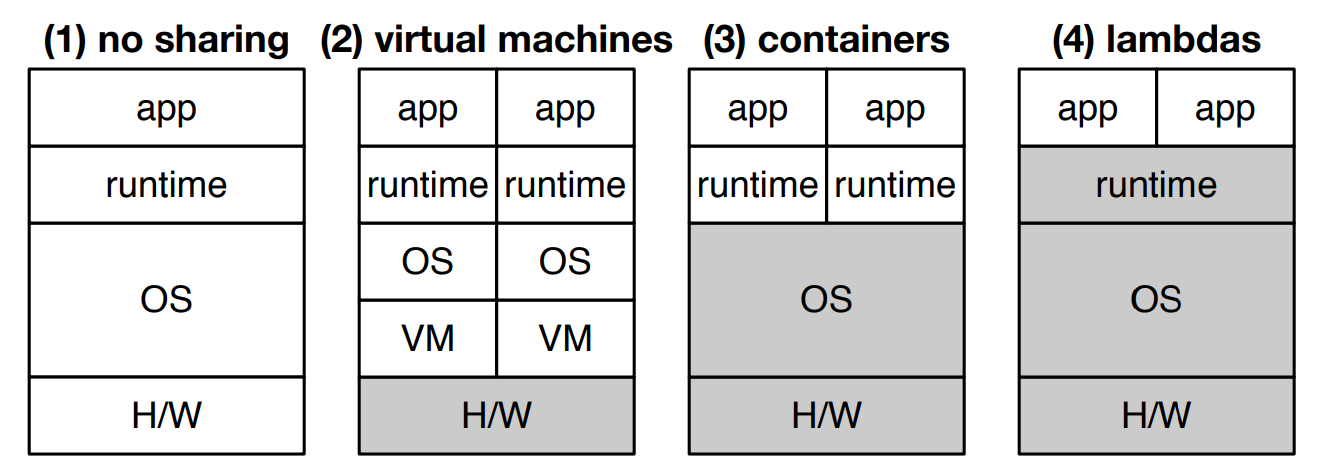
\includegraphics[width=0.7\textwidth]{serverlessSharing.png}
		\caption{Porównanie ilości warstw współdzielonych przez różne typy komponentów osadzonych w chmurze. \cite{openLambdaArticle}}
		\label{fig:serverlessSharing}
\end{figure}

Technologie serverless wciąż znajdują się w fazie rozwoju, jednak wyglądają bardzo obiecująco. Zgodnie z badaniem przytoczonym w artykule\cite{serverlessArticle}, podejście serverless może powodować oszczędności względem architektur monolitycznych oraz mikrousługowych na poziomie do 70.08\%. Powoduje również znaczną oszczędność czasu pracy nad projektem.\cite{serverlessMaddie}

\subsection*{Podsumowanie}

\subsubsection{Usługi FaaS}

\begin{itemize}
\item \textbf{AWS Lambda} -- pierwsza platforma tego typu. Obsługiwane języki: Java, Python, Node.js, C\#/.NET Core, Go
\item \textbf{Azure Functions} -- platforma serverless bazująca na WebJobs. Obsługiwane języki (bez uwzględniania wsparcia eksperymentalnego i poglądowego):
	\begin{itemize}
		\item w wersji 1.x: C\#, F\#/.NET Framework, Node.js 6
		\item w wersji 2.x (oficjalnie dostępnej od 24.09.2018 r. \cite{siteAzureFunctions2}): C\#, F\#/.NET Core 2, Node.js 8 \& 10
	\end{itemize}
\item \textbf{Google Cloud Functions} -- platforma serverless oficjalnie dostępna od sierpnia 2018 r. \cite{siteGoogleServerless} Obsługiwane języki: Java, Python
\end{itemize}

\subsubsection{Główne usługi wspierające tworzenie back-endu dla aplikacji mobilnych}
Tak jak w sekcji dotyczącej usług PaaS w oparciu o maszyny wirtualne (sekcja \ref{section:podejsciePaas}).

\subsubsection{Perspektywy}
\begin{itemize}
\item Mniejszy koszt utrzymania aplikacji przez brak konieczności zajmowania zasobów w oczekiwaniu na przychodzące zapytania.
\item Brak konieczności umiejętnego projektowania mikrousług.
\item Skalowanie pozbawione nadmiarowości.
\item Szybki czas wdrożenia aplikacji do chmury (2x szybciej niż mikrousługi) \cite{serverlessMaddie}
\end{itemize}

\subsubsection{Ograniczenia}
\begin{itemize}
\item Wady dziedziczą się z podejścia PaaS do tworzenia aplikacji w chmurze publicznej (sekcja \ref{section:podejsciePaas}, za wyjątkiem konieczności nauki projektowania mikrousług).
\item Utrudnienia w uruchamianiu dłużej trwających zadań.
\item Ograniczona możliwość testowania funkcji offline.
\end{itemize}



\section{Serverless bez przywiązania do platformy} 

Podczas gdy usługi FaaS w chmurach publicznych jawią się jako najtańsze oraz posiadające najmniejszą barierę wejścia do chmury, wciąż dziedziczą po innych rozwiązaniach typu PaaS starszy problem przywiązania do usługodawcy. Jest to dość istotny problem, biorąc pod uwagę to jaką popularność zdobył Docker oraz Kubernetes stanowiąc wybawienie od niego.

W literaturze przedmiotu znaleziono dwa projekty, które mają rozwiązać ten problem.

\subsection{Serverless Framework}

Jest to narzędzie do rozwijania i wdrażania funkcji w sposób oddzielający logikę konkretnego dostawcy usługi FaaS od sposobu pisania funkcji. Dzięki temu jeden kod jest gotowy do działania na różnych platformach (w tym Kubeless, o którym mowa w następnej sekcji). \cite{serverlessMaddie}

\begin{figure}[h]
	\centering
			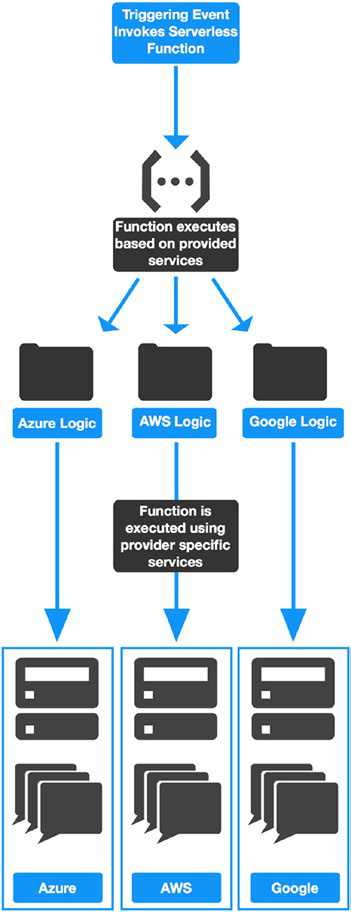
\includegraphics[width=0.4\textwidth]{serverless-framework.png}
		\caption{Oddzielenie logiki aplikacji od logiki dostawcy usługi FaaS przy pomocy Serverless Framework \cite{serverlessMaddie}}
		\label{fig:serverless-framework}
\end{figure}

Rozwiązanie problemu \textit{vendor lock-in} skutkuje następującymi ograniczeniami:
\begin{itemize}
\item Narzędzia będące nakładkami na inne narzędzia zawsze dążą do obsługiwania wspólnego mianownika tych narzędzi. Wyklucza to (lub znacząco utrudnia) użycie pewnych specyficznych usług typu PaaS danego dostawcy.
\item Konieczność uczenia się dodatkowego narzędzia.
\end{itemize}


\subsection{Kubeless}

Jest to framework działający na Kubernetes, pozwalający uruchomić mechanizm serverless podobny do tego spotykanego w usługach FaaS. \cite{distributedSystems} 

Kubeless obsługuje technologie: Python, Node.js, Ruby, PHP, Go, .NET, Ballerina. Funkcje tworzone z obrazów Dockera są w trakcie rozwoju.

Podstawowym ograniczeniem związanym z używaniem Kubeless jest konieczność zdobycia najpierw Kubernetes. Bez względu na to, czy będzie on zainstalowany na fizycznym serwerze czy maszynie wirtualnej (ręcznie albo przez KaaS), wciąż trzeba przede wszystkim zapewnić mu zasoby na których można go uruchomić. Eliminuje to zatem prawdopodobnie najważniejszą korzyść jaką wnosi serverless na chmurze publicznej, czyli brak stałych opłat za utrzymanie funkcji. Co prawda w Kubeless funkcja jest uruchomiona tylko przez chwilę, ale Kubernetes już działa cały czas.


\chapter{Analiza wyboru platformy dla aplikacji mobilnej}

\section{Opis projektu aplikacji mobilnej}

Pomysł na aplikację mobilną tworzoną w ramach pracy, to realny przykład aplikacji, dla której chmura może stanowić niezbędne wsparcie. Powody ku temu są następujące:
\begin{itemize}
\item do działania wymaga serwera,
\item komunikuje się używając REST-owego API,
\item działa w oparciu o treść tworzoną przez użytkowników,
\item w teorii ma szansę zyskać popularność, czyli może być wymagana zdolność do skalowania w górę.
\end{itemize}

\subsection{Geneza pomysłu}\label{section:genezaPomyslu}

Pomysł polega na stworzeniu nowatorskiej aplikacji służącej do zapisywania wydatków. Tego typu aplikacje dotychczas tworzone były z myślą o jednym użytkowniku i raczej nie wymagały do działania serwera. Z doświadczenia autorki pracy, takie podejście jest skuteczne do czasu, gdy mieszka się samemu, a wszystkie wydatki tworzy się z myślą o sobie. 

W przypadku gdy mieszka ze sobą więcej osób, liczby przestają cokolwiek mówić, gdyż może być tak, że jedna osoba robi więcej zakupów czy inna płaci rachunki. Powstają problemy jak się nawzajem rozliczać. Szczególnie biorąc pod uwagę, że różne kategorie wydatków można rozliczać w różny sposób, np.:
\begin{itemize}
\item wydatki na higienę, gdzie z części rzeczy korzystają wszyscy, a część służy konkretnym osobom,
\item wydatki na samochód, gdzie za naprawy mogliby płacić wszyscy użytkownicy po równo, a za paliwo zgodnie z użytkowaniem,
\item wydatki na rachunki, gdzie można ustalić, że osoba zarabiająca więcej będzie płaciła proporcjonalnie więcej,
\item wydatki na jedzenie, gdzie jedzenie dla jednej osoby może kosztować znacznie więcej niż dla drugiej.
\end{itemize}
Gdy gospodarstwo domowe liczy więcej osób, wzajemne rozliczenia stają się skomplikowane. Trudno wówczas prowadzić budżet domowy, kontrolować gdzie ,,wyciekają'' pieniądze. Można starać się, aby wydatki były zapisywane na jednym komputerze, można pewne obliczenia przeprowadzić ręcznie. Nie zapewnia to jednak wygody oddzielenia własnych wydatków od wydatków innych, a także nie umożliwia sprawdzania np. ile wynoszą wydatki na jedzenie w tym miesiącu.

Biorąc pod uwagę powyższe, idealnym rozwiązaniem problemu zapisywania wydatków przez kilka osób byłaby aplikacja, która umożliwiłaby połączenie kilku użytkowników w grupę i przy pomocy serwera przeprowadzałaby wszystkie potrzebne obliczenia. Gwarantowałoby to niespotykaną wcześniej precyzję w rozliczeniach, przy jednoczesnej prostocie obsługi. 

Do obsługi wystarczyłaby jakakolwiek aplikacja kliencka zdolna do połączenia z Internetem. Serwer zadbałby o właściwą synchronizację pomiędzy instancjami aplikacji. Aby umożliwić precyzyjne rozliczenia, dodawanie wydatku powinno umożliwić wyszczególnienie, że należy do kategorii, w której panuje określony sposób rozliczeń. 

Jest możliwe ułatwić tę czynność przez rozpoznawanie obrazu, gdzie podstawowe parametry (cena na paragonie, data zakupu, nazwa sklepu) byłyby wczytywane automatycznie. Z doświadczenia autorki w zapisywaniu dodatków wynika, że zazwyczaj prawie wszystkie pozycje na paragonie odnoszą się do jednej kategorii. Aby wygodnie wyszczególnić pojedynczą rzecz na paragonie, wystarczy odjąć ją od ceny całkowitej i przypisać do innej kategorii. Możliwość wyszczególnienia wydatków z danego paragonu byłaby sporym ułatwieniem.

Również z doświadczenia autorki spory problem stanowi rozliczanie wydatków na jedzenie. Trudno wyznaczyć model, w którym owo rozliczenie przeprowadzone jest jednocześnie sprawiedliwie oraz wygodnie. Możliwym rozwiązaniem, będącym elementem pomysłu na aplikację, byłoby automatyczne tworzenie przeliczników dla kategorii ,,jedzenie'', bazując na wprowadzonych danych takich jak: waga, wiek, płeć, wzrost i poziom aktywności fizycznej u danej osoby. Wykorzystując siłę serwera w chmurze, wszystkie potrzebne obliczenia byłyby przeprowadzone automatycznie.

Kolejną rzeczą będącą utrapieniem tradycyjnych aplikacji są wycieczki zagraniczne i wydatki w obcej walucie. Trudno w takich sytuacjach podtrzymywać kontrolę nad tym, ile ma się pieniędzy, jeśli część występuje w obcej walucie. Dlatego pomysł uwzględnia także obsługę różnych walut.

Tak skonstruowana aplikacja praktycznie nie wymagałaby większego wysiłku niż tradycyjne programy do zapisywania wydatków. Za to posiadając dodatkowe informacje byłaby w stanie generować wiele przydatnych raportów, np.:
\begin{itemize}
\item ile wydaje się jako gospodarstwo domowe w danej kategorii,
\item ile dana osoba wydaje na ubrania,
\item ile wspólnie wydaje się na życie,
\item ile dana osoba wydaje na jedzenie,
\item w których sklepach najczęściej się wydaje pieniądze,
\item ile dana osoba lub wszyscy razem posiadają pieniędzy w jakich walutach.
\end{itemize}

\subsection{Typowy projekt dla chmury}

Opisany w sekcji \ref{section:genezaPomyslu} pomysł stanowi przykład typowego projektu informatycznego. Rozwiązuje problem życia codziennego przez umiejętne zebranie informacji, przetworzenie jej i zwrócenie wartościowych wyników. 

Jednocześnie nie jest to pomysł czysto teoretyczny, czyli taki, z jakim często można mieć styczność przerabiając różne samouczki od programowania. Tego rodzaju projekty są często zbyt uproszczone, by pozwolić zetknąć się z rzeczywistymi problemami. Nie jest to sztandarowy program do napisania, taki jak ,,lista zadań'', który został już przerobiony przez innych pod każdym możliwym kątem.

Realizacja tego pomysłu nie byłaby możliwa bez serwera. Serwer można teoretycznie utworzyć na tradycyjnej infrastrukturze niezgodnej z modelem chmury. Wówczas niestety aplikacji grozi tzw. ,,syndrom Naszej-Klasy'' (nazwany tak w książce \textit{,,Windows Azure. Wprowadzenie do programowania w chmurze''}), gdzie autor aplikacji sam nie przewiduje jej nagłego wzrostu popularności. Sukces staje się wtedy zwiastunem klęski, ze względu na wdrożenie aplikacji w sposób niepozwalający na obsługę większego ruchu. Zirytowani użytkownicy odwracają swoje zainteresowanie od aplikacji, która ma problemy z dostępnością. \cite{windowsAzureWprowadzenie} Zależność tę widać na rysunku \ref{fig:nasza-klasa}.

\begin{figure}[h]
	\centering
			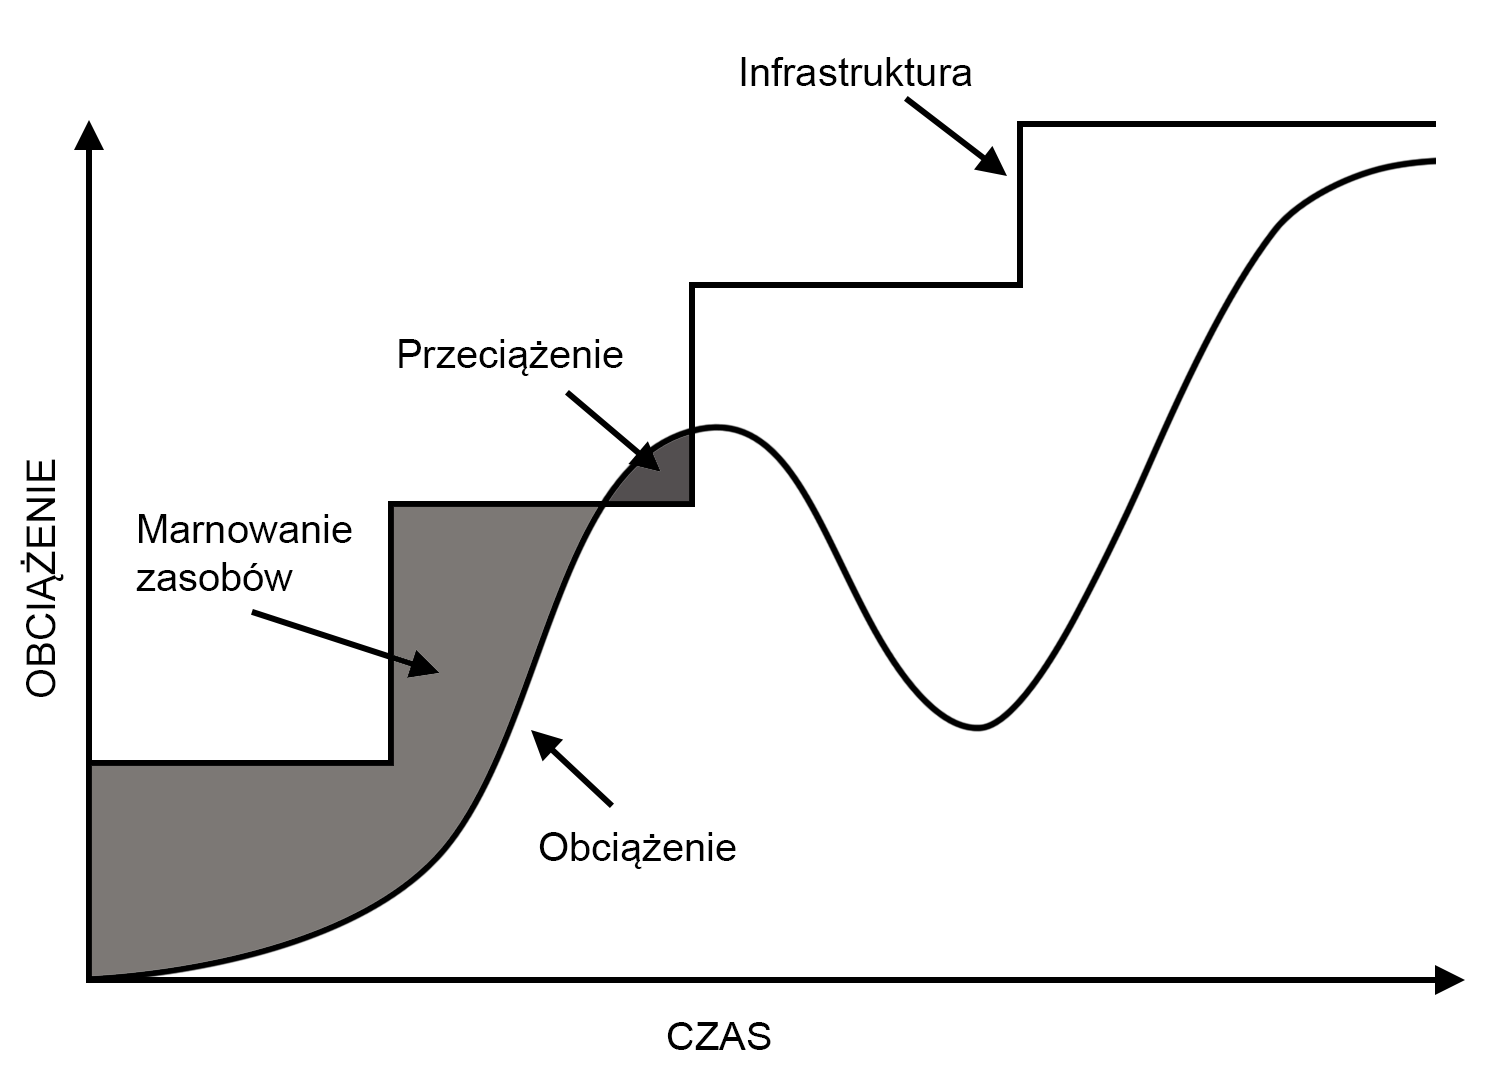
\includegraphics[width=0.85\textwidth]{nasza-klasa.png}
		\caption{Wykres obrazujący problem tradycyjnego podejścia do skalowania aplikacji \cite{windowsAzureWprowadzenie}}
		\label{fig:nasza-klasa}
\end{figure}

Biorąc pod uwagę powyższe, wykorzystanie chmury okaże się przydatne właśnie w momencie, kiedy aplikacja okaże się sukcesem. Jeśli aplikacja nie ma szansy na sukces, nie ma sensu jej w ogóle  wdrażać. Jeśli ma szanse na sukces, to lepiej zapewnić jej skalowalne środowisko.

Ważnym elementem skalowalności aplikacji jest jej budowa. Nawet aplikacja wdrożona w chmurze, jeśli zostanie stworzona w sposób tradycyjny, jest narażona na problemy ze skalowalnością. Tradycyjnie większą ilość zasobów osiągało się przez skalowanie wertykalne, czyli wymianę serwera na taki o lepszych parametrach sprzętowych (rysunek \ref{fig:skalowanie-wertykalne}). Niestety specjalistyczne zasoby komputerowe o wysokiej mocy są drogie, a i one mają swoje granice. 

\begin{figure}[h!]
	\centering
			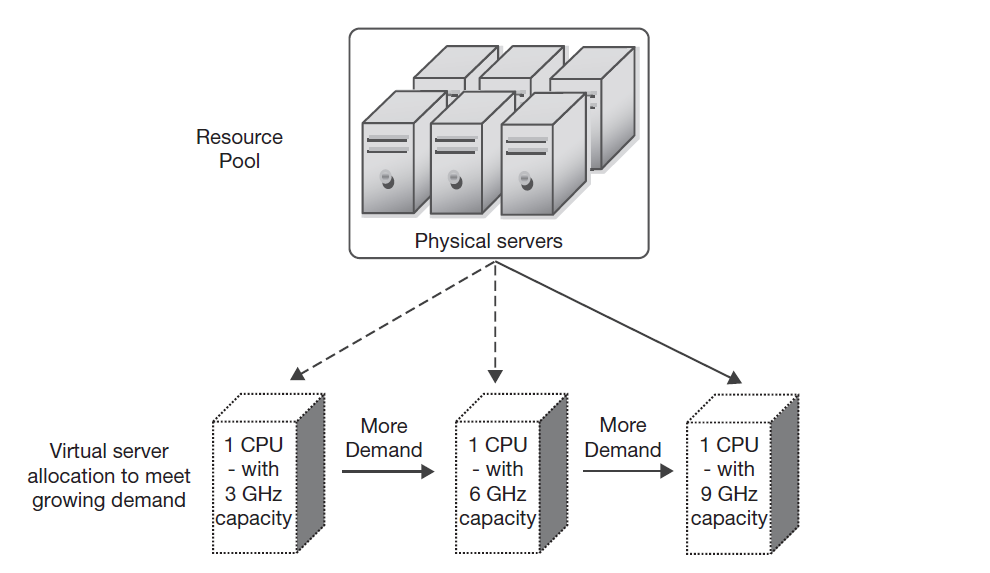
\includegraphics[width=\textwidth]{skalowanie-wertykalne.png}
		\caption{Skalowanie wertykalne -- wraz z rosnącym zapotrzebowaniem wymiana serwera na taki z lepszymi parametrami \cite{ccCambridge}}
		\label{fig:skalowanie-wertykalne}
\end{figure}

Z pomocą przychodzi skalowanie horyzontalne. Ponieważ pozwala połączyć siły wielu komputerów, które pod względem zasobów mogą być przeciętne i tanie (rysunek \ref{fig:skalowanie-horyzontalne}). Nie istnieje wówczas problem ze skalowalnością ani z przerwą w dostarczaniu usług. Możliwość skalowania horyzontalnego wymaga użycia odpowiedniej architektury aplikacji.

\begin{figure}[h!]
	\centering
			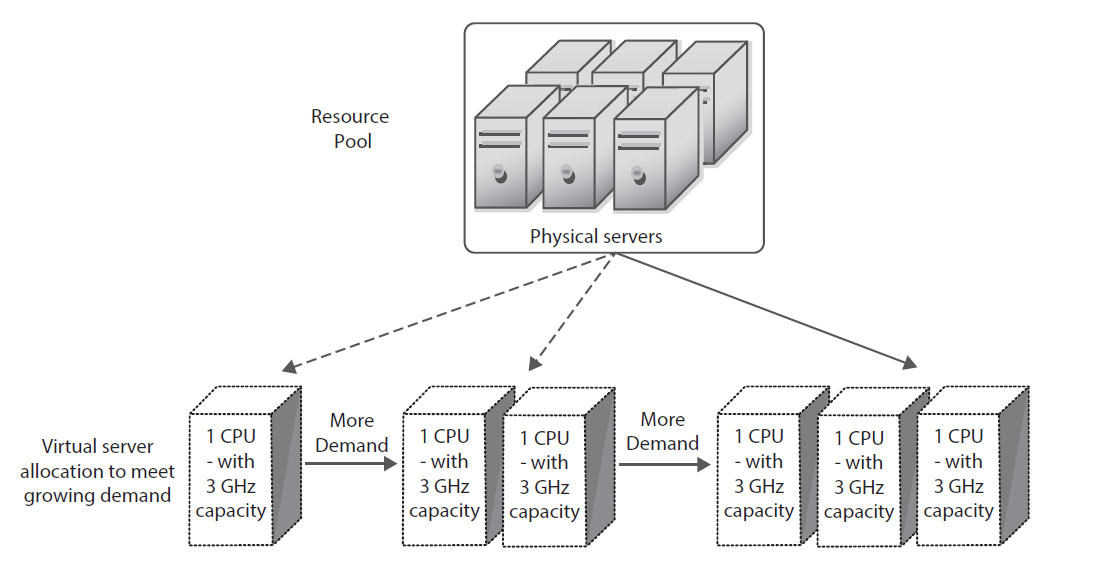
\includegraphics[width=\textwidth]{skalowanie-horyzontalne.png}
		\caption{Skalowanie horyzontalne -- wraz z rosnącym zapotrzebowaniem dokładanie serwerów o tej samej mocy \cite{ccCambridge}}
		\label{fig:skalowanie-horyzontalne}
\end{figure}

Chmura idealnie nadaje się do skalowania horyzontalnego. Tworzona z setek tysięcy maszyn daje możliwość obsłużenia nawet nadspodziewanie wysokiego ruchu. Z kolei usługi chmurowe wspomagają proces tworzenia aplikacji typu \textit{cloud native}, tworzonych za pomocą mikrousług i korzystających z baz NoSQL.

Kolejnym ważnym aspektem, dla którego warto rozważyć użycie chmury, jest dostępność usług wykorzystujących uczenie maszynowe do np. rozpoznawania obrazu, a także usług związanych z przetwarzaniem dużej ilości danych. W dłuższej perspektywie ułatwienia takie jak automatyczne czytanie danych ze zdjęcia paragonu lub możliwość wykonania analizy dużego zbioru danych mogą stanowić dużą wartość dodaną.

Wymienione powyżej przesłanki wskazują na to, że omawiany projekt posiada cechy typowego projektu informatycznego i z powodzeniem obrazuje sens wykorzystania chmury do tworzenia nawet eksperymentalnych projektów.

\section{Wymagania dotyczące wyboru podejścia oraz chmury}



\section{Analiza}

\subsection{Wybór podejścia}

\subsection{Wybór chmury}

\subsection{Podsumowanie analiz}





\chapter{Opis wdrożenia aplikacji zgodnie z kandydatką nr 1 }
 
\chapter*{Podsumowanie}
 
 
 
 
\addcontentsline{toc}{chapter}{Spis rysunków}
\listoffigures

\addcontentsline{toc}{chapter}{Spis tabel}
\listoftables



\addcontentsline{toc}{chapter}{Bibliografia}
\selectlanguage{polish}
\printbibliography
 


\end{document}
